\documentclass[lettersize,journal]{IEEEtran}
\usepackage{amsmath,amsfonts}
\usepackage{algorithmic}
\usepackage{algorithm}
\usepackage{array}
\usepackage[caption=false,font=normalsize,labelfont=sf,textfont=sf]{subfig}
\usepackage{textcomp}
\usepackage{stfloats}
\usepackage{url}
\usepackage{verbatim}
\usepackage{graphicx}
\usepackage{xcolor}
\usepackage{cite}
\usepackage{multirow}
\usepackage[utf8]{inputenc}
\usepackage{lscape} 
\hyphenation{op-tical net-works semi-conduc-tor IEEE-Xplore}

\begin{document}

\title{Framework for Assurance of Emergent Behaviour for use in Autonomous Robotic Swarms}

\author{Author1\_Name, Author2\_Name, ...AuthorN\_Name,
\thanks{Author1 and Author2 are with the Department of Dep1\_Name (email: , )}
\thanks{AuthorN is with the Department of Dep2\_Name (email: )}}
%\thanks{Manuscript received April 19, 2021; revised August 16, 2021.}}
% The paper headers
\markboth{Journal of \LaTeX\ Class Files,~Vol.~14, No.~8, August~2021}%
{Shell \MakeLowercase{\textit{et al.}}: A Sample Article Using IEEEtran.cls for IEEE Journals}

%\IEEEpubid{0000--0000/00\$00.00~\copyright~2021 IEEE}
% Remember, if you use this you must call \IEEEpubidadjcol in the second
% column for its text to clear the IEEEpubid mark.

\maketitle

\begin{abstract}
	Abstract of the paper.
\end{abstract}

\begin{IEEEkeywords}
	Assurance, swarm robotics, trustworthiness, safety, transparency, ethics, autonomous systems
	%Swarm Robotics, Acceptability and Trust, Autonomous Agents
\end{IEEEkeywords}

\section{Introduction}\label{introduction}
The main contribution of this paper is a novel framework for assurance of emergent behaviour for use in autonomous robotic swarms based on the AMLAS, SACE* and SOCA* guidance (* under consideration). We illustrate the framework using a public cloakroom case study. 

%\\\noindent\textbf{\textit{[Author General Guidelines: please write as a paper not as a Guidance like AMLAS; Please do not use AERoS word]}}\\


\section{Background and Related Work}\label{background-relatedwork}

\subsection{Background}\label{background}

\subsubsection{Specification Challenges and Standards}
%\newline With respect to swarms, the overall behaviours of a swarm are not explicitly engineered in the system, but they are an emergent consequence of the interaction of individual agents with each other and the environment.
%This emergent functionality poses a challenge for specification. 
%\newline How do you ensure safety or any other extra-functional property of a swarm where the swarm’s behaviour is an “emergent” consequence of the interaction of individual agents with each other and their environment?
%Swarm behaviours:
%\newline Aggregation 
%\newline Coherent ad-hoc network
%\newline Information retrieval
%\newline Taxis towards pick up and delivery areas of boxes
%\newline Obstacle avoidance
%\newline Object organization
%
%\textit{IEEE P7001} standard describes measurable, testable levels of transparency for autonomous systems so that they can be objectively assessed and levels of compliance determined\cite{IEEE-P7001}. 
%This standard outlines five stakeholder groups, and for each group it explains the structure of the normative definitions of levels of transparency. 
%\textit{IEEE P7001} can be applied to assess the transparency of an existing system using a process of System Transparency Assessment, or to specify transparency requirements for a system prior to its implementation (System Transparency Specification).
%The 5 stakeholders are end users, general public and bystanders, safety certification agencies and auditors, incident/accident investigators, expert advisors.
%
%In service robotics, ISO 13482 covers the hazards presented by the robots and devices for applications in non-industrial environments for providing services. 
%ISO 23482-1 and ISO 23482-2 standards extend ISO 13482 with guidance and methods that can be used to test personal care robots.
%On the other hand, in the industrial sector, ISO 10218-1 and ISO 10218-2 provide safety requirements for industrial robots and their integration.
%Meanwhile, ISO/TS 15066 provides safety requirements for collaborative industrial robot systems and work environment. 
%Although these industry standards focus on ensuring safety of robots at the individual robot level, they do not ensure safety or any other extra-functional property at the swarm level, which is a limitation.
%
%This Figure shows a categorization of robots by ISO. 
%Identifying which robot category the individual robots of the cloakroom is important because different legal and regulatory requirements apply to different robot categories.
%The “service robot” contains most robot categories, except industrial robot. 
%These are: household robots, medical robots and personal care robots.
%The individual robots of the cloakroom better fit into the “mobile servant robots” category, which is a type of personal care robot under service robots.
%A mobile servant robot is a personal care robot capable of travelling to perform serving tasks in interaction with humans, e.g. handling objects or exchanging information [ISO 13482:2014, 3.14].
\vspace{2mm}

\subsubsection{Robotic Swarms}
%\noindent Autonomous
%\\ \noindent Large Number of agents (10+)
%\\ \noindent Relatively incapable individuals
%\\ \noindent Restrained Homogeneity
%\\ \noindent Minimal communication capabilities (Decentralised)
\vspace{2mm}

\subsubsection{Case Study}

\vspace{2mm}
\noindent\textbf{\textit{\newline[Author Guidelines: Please use the cloakroom case study to illustrate the framework in Section III. If the examples in cloakroom case study are not sufficient, other swarm use cases listed below can be considered.]}}

\paragraph{\textbf{Cloakroom}\label{ex:cloakroom}}
The case study describes a public cloakroom where swarm of robots assist customers looking to deposit their jackets at an event \cite{Jones2020}. 
It describes cases where customers are depositing jackets, handing a jacket to a robot for storing, and retrieval of jackets back to the customer. 

\paragraph{Other Swarm Use Cases}
\textbf{\\Fault detection, diagnosis and recovery – Monitoring fires in a natural environment}. Fault detection model shall be trained to high level of accuracy. Thresholds for fault tolerance shall be set appropriately such that misclassification of a fault is a rare event. An agent experiencing minor faults shall not be immediately removed, should the fault not impact the task at hand. \\
\textbf{\noindent Social swarm – Brainstorming at an event}. Humans follow robots which cluster based on input. Minimise blocking paths of other humans and agents. Maintain situational awareness of humans and agents in the environment. Before the task, provide a clear explanation of the steps of the activity. Clear guidance during the task. Provide information about how the swarm/robot works.

\noindent See research paper ``Mutual shaping in swarm robotics: User studies in fire and rescue, storage organization, and bridge inspection" \cite{Carrillo-Zapata2020}.

\subsection{Related Work}\label{relatedwork}

\subsubsection{Assurance of Machine Learning in Autonomous Systems (AMLAS)}
%\cite{Hawkins2021}
\textit{Assurance of Machine Learning for use in Autonomous Systems (AMLAS)} provides guidance on how to systematically integrate safety assurance into the development of machine learning components based on offline supervised learning \cite{AMLAS2021}. 
AMLAS provides an explicit and structured safety case that the system is safe to operate in its intended context of use. 
AMLAS contains six stages, and the assurance activities are performed in parallel to the development of machine learning component. 
The process is iterative by design and feedback is used to update previous stages. 

\subsubsection{Safety Assurance of Autonomous Systems in Complex Environments (SACE)}
\cite{SACE2022}

\subsubsection{Societal Acceptability of Autonomous Systems (SOCA)}
\cite{Porter2022,McDermid2021}

\section{Framework}\label{framework}

\subsection{Overview of Framework} \label{framework-overview}
%Simple algorithms are executed by individuals.
%These simple behaviours performed by large numbers of agents build to emergent behaviours.
%The adaptivity provided by emergence requires assurance. 
%
%Safety Assurance Process based on AMLAS targeting robotic swarms:
%Emergent behaviour
%Failure conditions that the output of an individual robot or a robot in the neighbourhood makes to potential swarm-level hazards.
%
%Scope of current study:
%Looking purely at inherent swarm qualities and the adaptation that stems from these.
%Developing individual behaviours which when combined create an adaptive emergence.
%Machine/Reinforcement Learning should not be considered at this time.
%We may expand to ML/RL for individuals. (Application of AMLAS to individuals once AMLAS has been applied to the swarm)
\vspace{2mm}

%\subsection{Stage 1: EB Safety Assurance Scoping} \label{framework-stage1}
%\noindent \textbf{\textit{[Lead:  WP1]}}\\
%\noindent\textbf{\textit{[Author Guidelines: 900–1800 words / 1–2 pages (maximum); \\Format/structure: Describe adapted AMLAS activities, inputs and outputs using cloakroom case study examples. Activities: 1, 2; Inputs: A, B, C, D, F; Outputs: E, G]}}\\
%See Fig.~\ref{amlas-a-stage1}
%\begin{figure*}
%	\centering
%	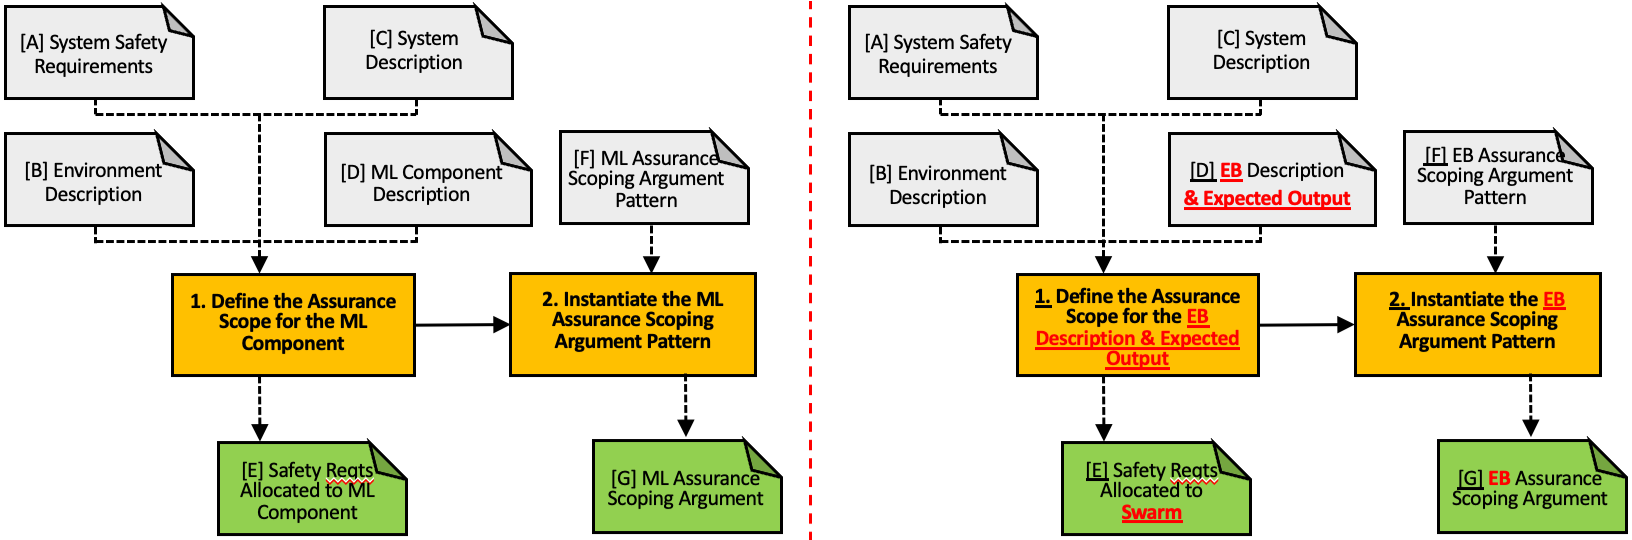
\includegraphics[width=1.0\textwidth]{figures/amlas-a-stage1.png}
%	\caption{Adapted AMLAS emergent behaviour assurance scoping process (right).}
%	\label{amlas-a-stage1}
%\end{figure*}

\subsection{Stage 1: EB Safety Assurance Scoping} \label{framework-stage1}
In this study, we look at inherent swarm qualities and the adaptation that arises from these qualities. 
In a swarm, individual robots execute simple behaviours or algorithms, and these simple behaviours when performed by a large number of agents build to form \emph{emergent behaviours} (EB). 
%These simple behaviours performed by large numbers of agents build to emergent behaviours.
%For this, we will look into developing individual behaviours which when combined create an adaptive emergence. 
The adaptivity provided by this emergence requires us to provide \textit{assurance} (e.g. safety assurance). 
At present, our study does not consider machine learning components of individual agents. Instead, these will be considered as part of future work once AMLAS has been applied to the swarm.
%However, we may consider this later once AMLAS has been applied to the swarm.

The adapted Stage 1 contains two activities which are performed to define the safety assurance scope for the swarm (see Fig.~\ref{amlas-a-stage1}).  
As part of activity 2, the artefacts generated from Stage 1 are used to instantiate the EB safety assurance scoping argument pattern. \\

\noindent \textbf{Activity 1: Define the safety assurance scope for the EB description and expected output}

The required inputs to Stage 1 are the system safety requirements ([A]), the operating environment [B], the system description [C], and a description of the EB and expected output ([D]). 
Inputs A, B, C and D will be used to determine the safety requirements which are allocated to the swarm. 
The requirements defined in Stage 1 are independent of any EB technique or metric.
Instead, these requirements reflect the need for the swarm to perform safely with the system regardless of the deployed technology. 
The output of this activity is the safety requirements that are allocated to the swarm [E]. 
\begin{figure}[!t]
	\centering
	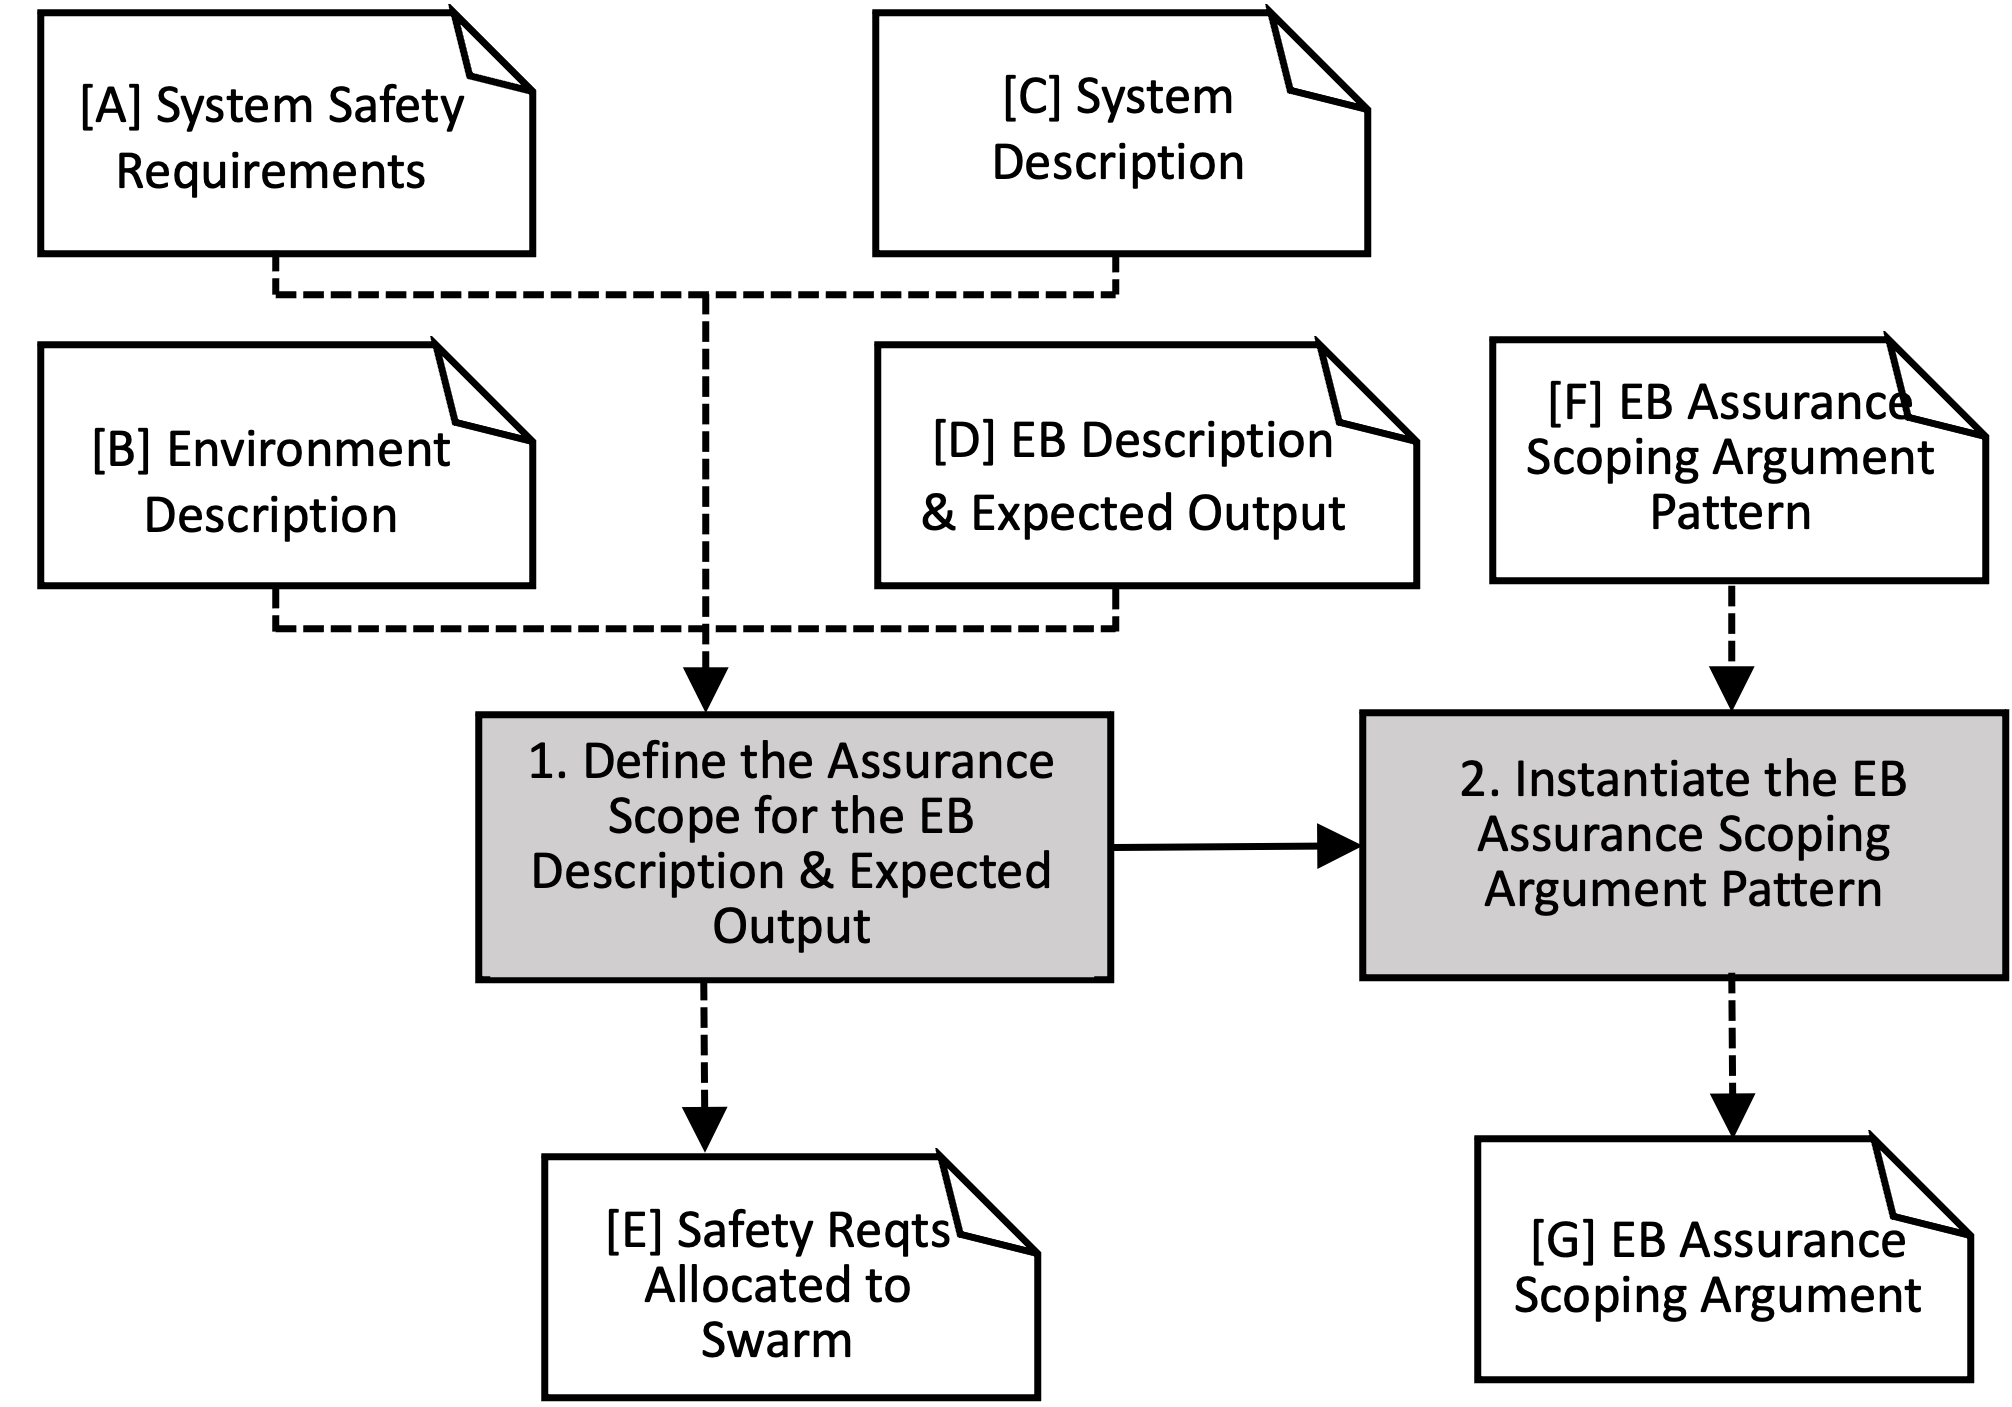
\includegraphics[width=0.5\textwidth]{figures/amlas-a-stage1-v2.png}
	\caption{Stage 1: Adapted AMLAS emergent behaviour assurance scoping process.}
	\label{amlas-a-stage1}
\end{figure}
\\

\noindent \textbf{Artefact A -- System safety requirements: }
The system safety assessment process generates the safety requirements of the swarm, which covers identification of hazards and risk analysis. 
As illustrated in Fig.~\ref{failure-events}, this can be shown in the form of concrete failure conditions from an individual robot propagating through the swarm neighbourhood, resulting in swarm-level hazards. 
Although this has been illustrated as a simplified linear chain of events, in reality this represents a complex sequence which can be difficult to distil into distinct events and cause.

With respect to hazard identification and risk analysis performed in our study, in the \textit{cloakroom} use case, a key hazard is the blocking of critical paths. 
This can result in humans or other agents in the swarm unable to travel to urgent locations in a safe manner. 

In the \textit{monitoring fires in a natural environment} use case, a considerable hazard can be presented should a critical fault go undetected. This can result in swarm operating with critically faulty agents resulting in the emergence of unsafe behaviour. The labelling of faults does, however, require caution and a level of trade off. Should a fault be misdiagnosed, for example, a minor fault being labelled as a critical fault (e.g. a minor reduction of the wheel speed labelled as full motor failure). The system or user may end up removing key agents from the swarm, resulting in significant loss of performance and efficacy in the swarms task.\\ 

\begin{figure}[!t]
	\centering
	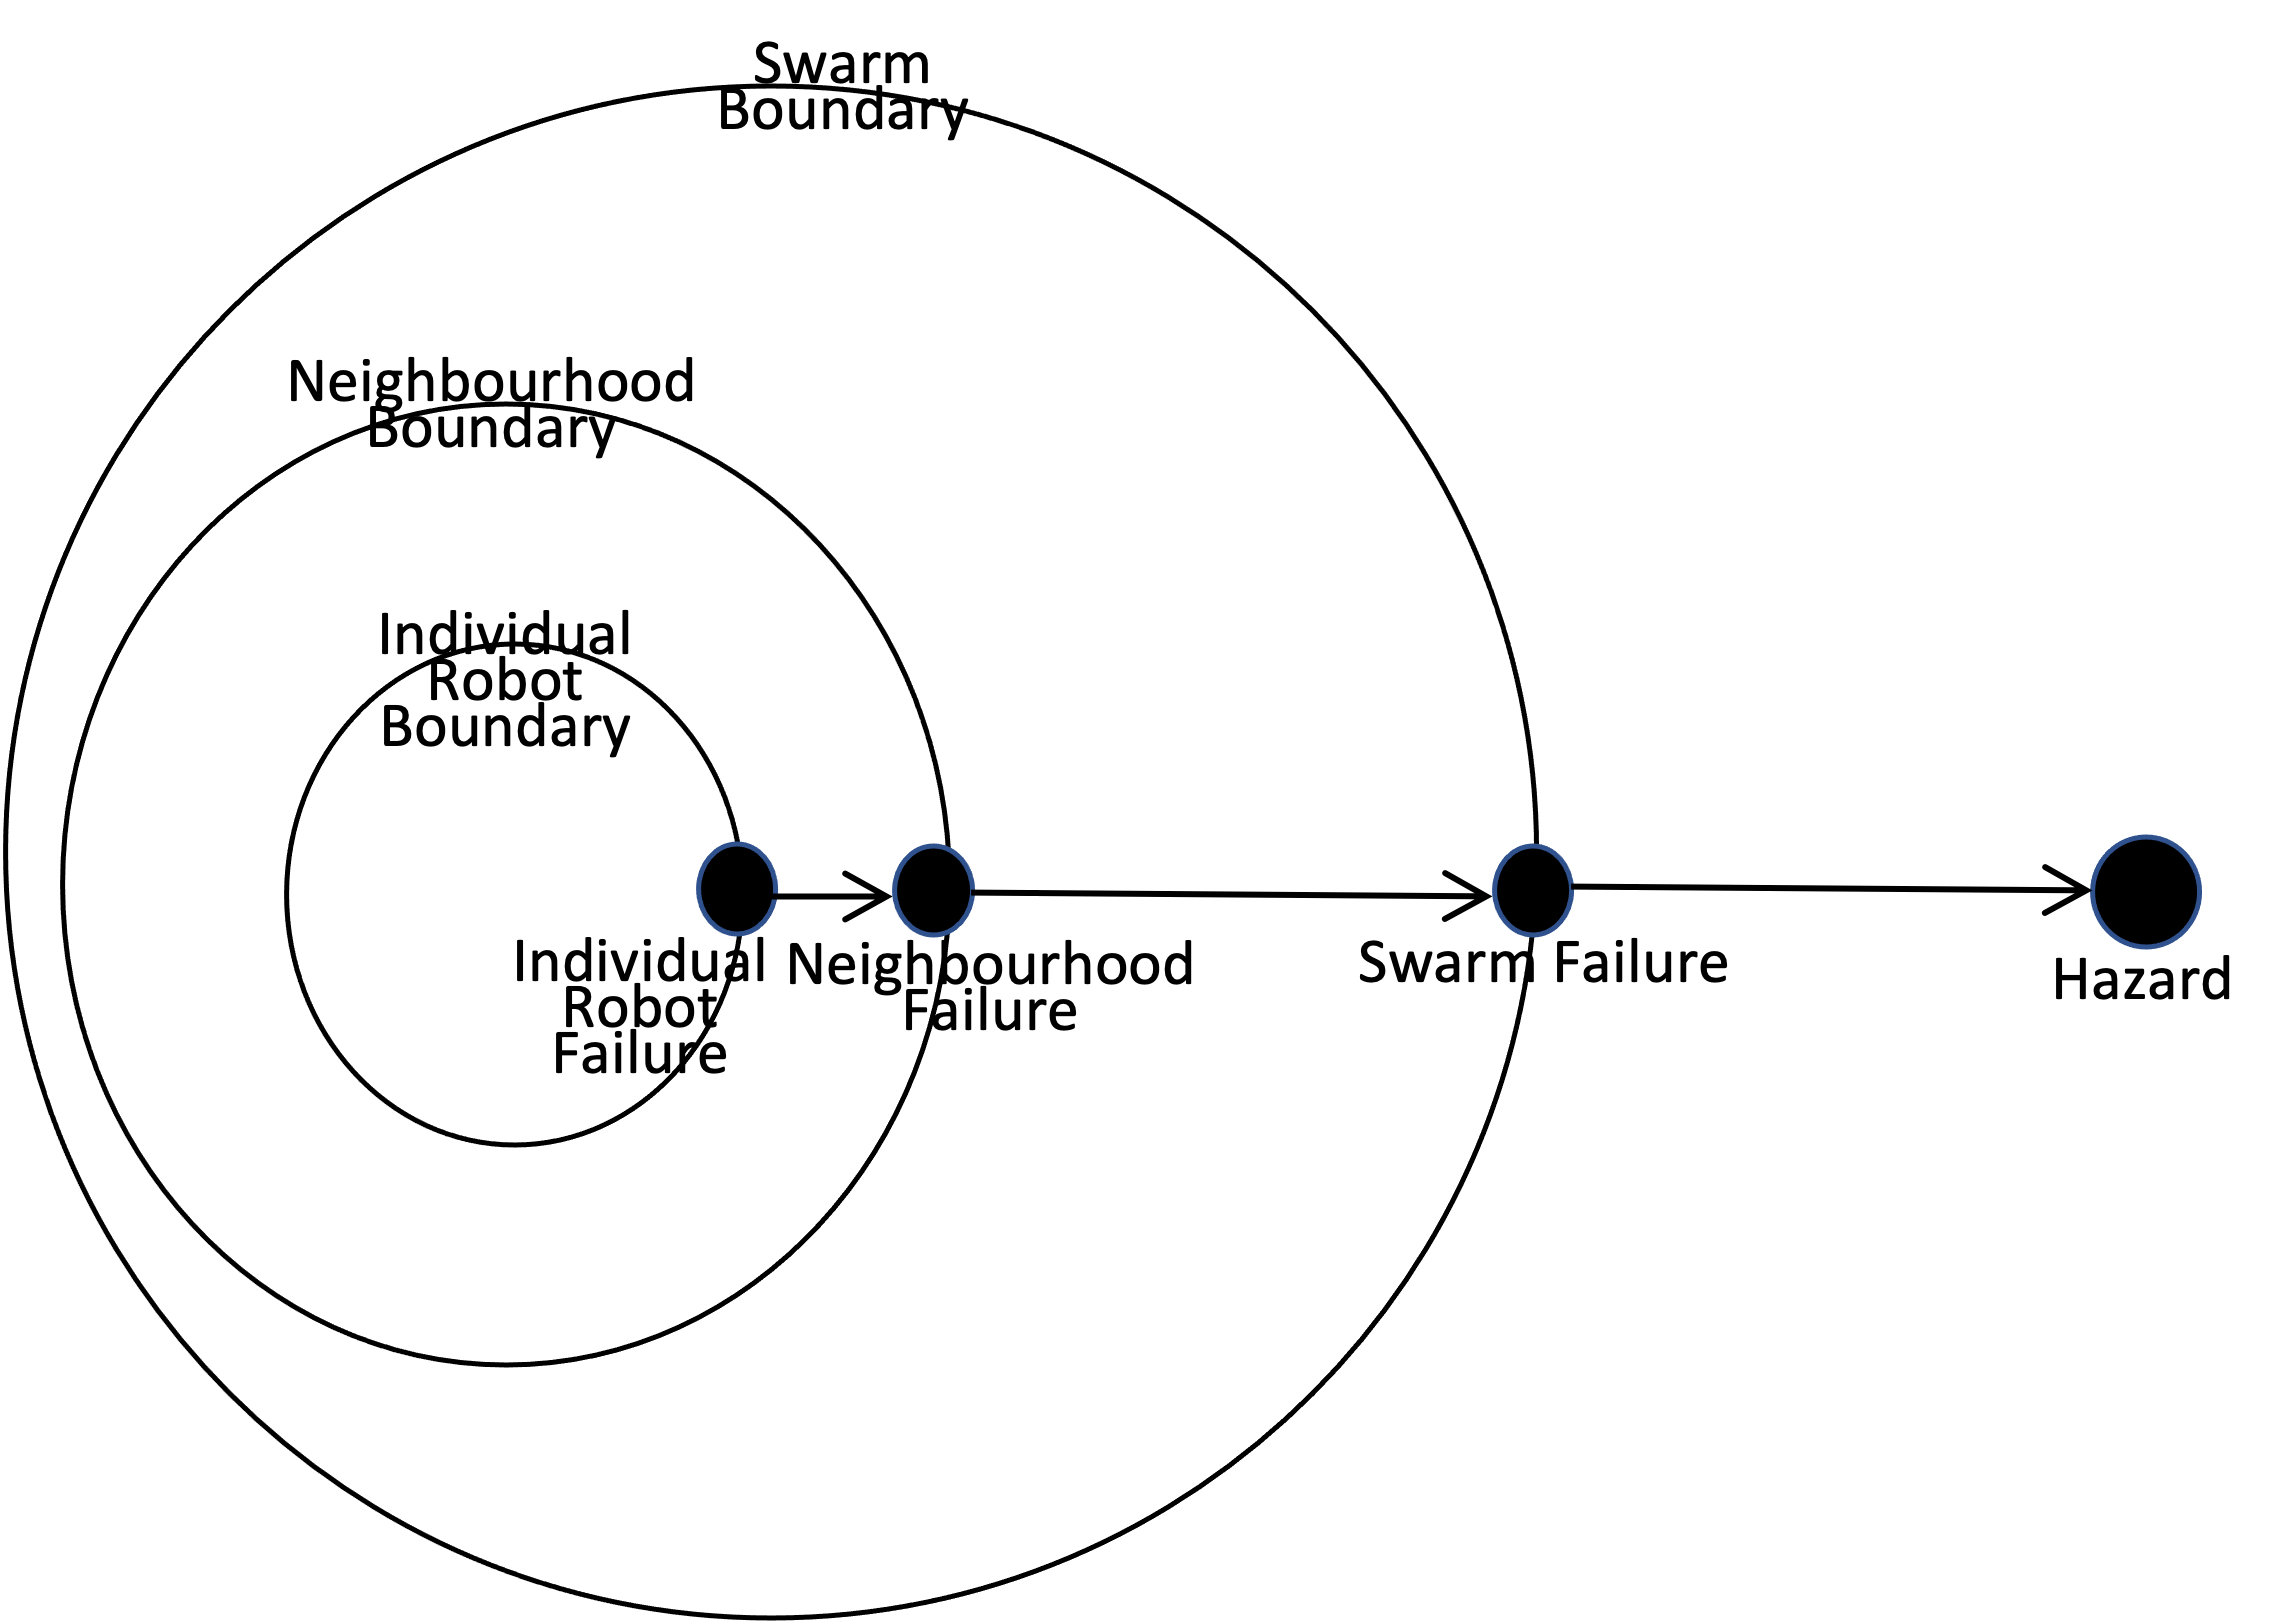
\includegraphics[width=0.5\textwidth]{figures/stage1-failureevents.png}
	\caption{Failure conditions in a swarm [adapted from DO-178C, AMLAS].}
	\label{failure-events}
\end{figure}

\noindent \textbf{Artefact B -- Environment description: }
As in AMLAS guidance, when allocating safety requirements to the swarm, it is essential to consider the system environment, which is represented by Artefact B. 
Based on the different use cases considered in our study, we can provide a description of their environments as follows.
\begin{itemize}
	\item \textit{A swarm of robotic agents collecting and delivering jackets, stored in small box-like containers within a cloakroom}. Agents are required to navigate a public space between collection and delivery points of jackets. Agents use local communication, perception, and data to form an emergent system of navigation that allows them to easily traverse the public space between jacket collection and delivery points.
	\item \textit{A swarm of UAVs monitoring wildfire risks in a natural environment}. Here, agents will be required to stay within communication range of each other, effectively covering the search area and accurately detecting risks of fire.
	\item \textit{Social swarm – brainstorming at an event}. Humans input their opinions on agents which then cluster based on the input. [Humans follow the agent they interacted with and user groups emerge in the process.]\\
\end{itemize}

\noindent \textbf{Artefact C -- System description: }
To describe our logistics use case, we must consider three inputs: sensor availability, neighbourhood data, and swarm parameters. 

In this instance, the \textit{sensors} available to agents might be: cameras (multiple), Bluetooth communication devices, and light detection and ranging systems (see Fig.~\ref{system-description}). 

The neighbourhood data of the swarm can be specified through the communication systems available to agents, in this case Bluetooth. Through the use of the short range communication available to them, we can assume agents have access to neighbourhood data such as: the approximate position of local agents, current behaviour statuses, an approximate history of box movement, and the amount of time deployed. 

As for the swarm level parameters, we can consider options specified by a user i.e. the number of agents deployed, the maximum speed of agents, and the number of agents allowed to be active at a time.

Once we have defined these three inputs they are fed to the individual agents to instruct their behaviour. This behaviour, once enacted by the multiple agents, produces a swarm level emergence as the individuals interact with one another and their environment.

\begin{figure}
	\centering
	
\includegraphics[width=0.4\textwidth]{figures/stage1-systema.png}
	\caption{System description.}
	\label{system-description}
\end{figure}

\noindent \textbf{Artefact D -- EB description and expected output: }
%This artefact describes the role and scope of the component within the system of which it is part, and the interfaces to which it is exposed.
By expected output here, we mean the gains that can arise from the system by deploying multiple agents.
%Let us consider the type and configuration of the emergent behaviour. 
For our logistics use case, the output is a collaborative system capable of collecting, sorting and redelivering jackets in a public setting. 

To achieved this output, the emergent behaviour of the system needs to be manually engineered by a swarm engineer with consideration to the available sub-behaviours within an agent and the constraints outlined in the system description.\\
%

\noindent \textbf{Activity 2: Instantiate the EB assurance scoping argument pattern}

\noindent \textbf{Artefact F -- EB Safety assurance scoping argument pattern: }
The argument pattern relating to this stage is shown in Fig.~\ref{stage1-ap}. 
\begin{figure}
	\centering
	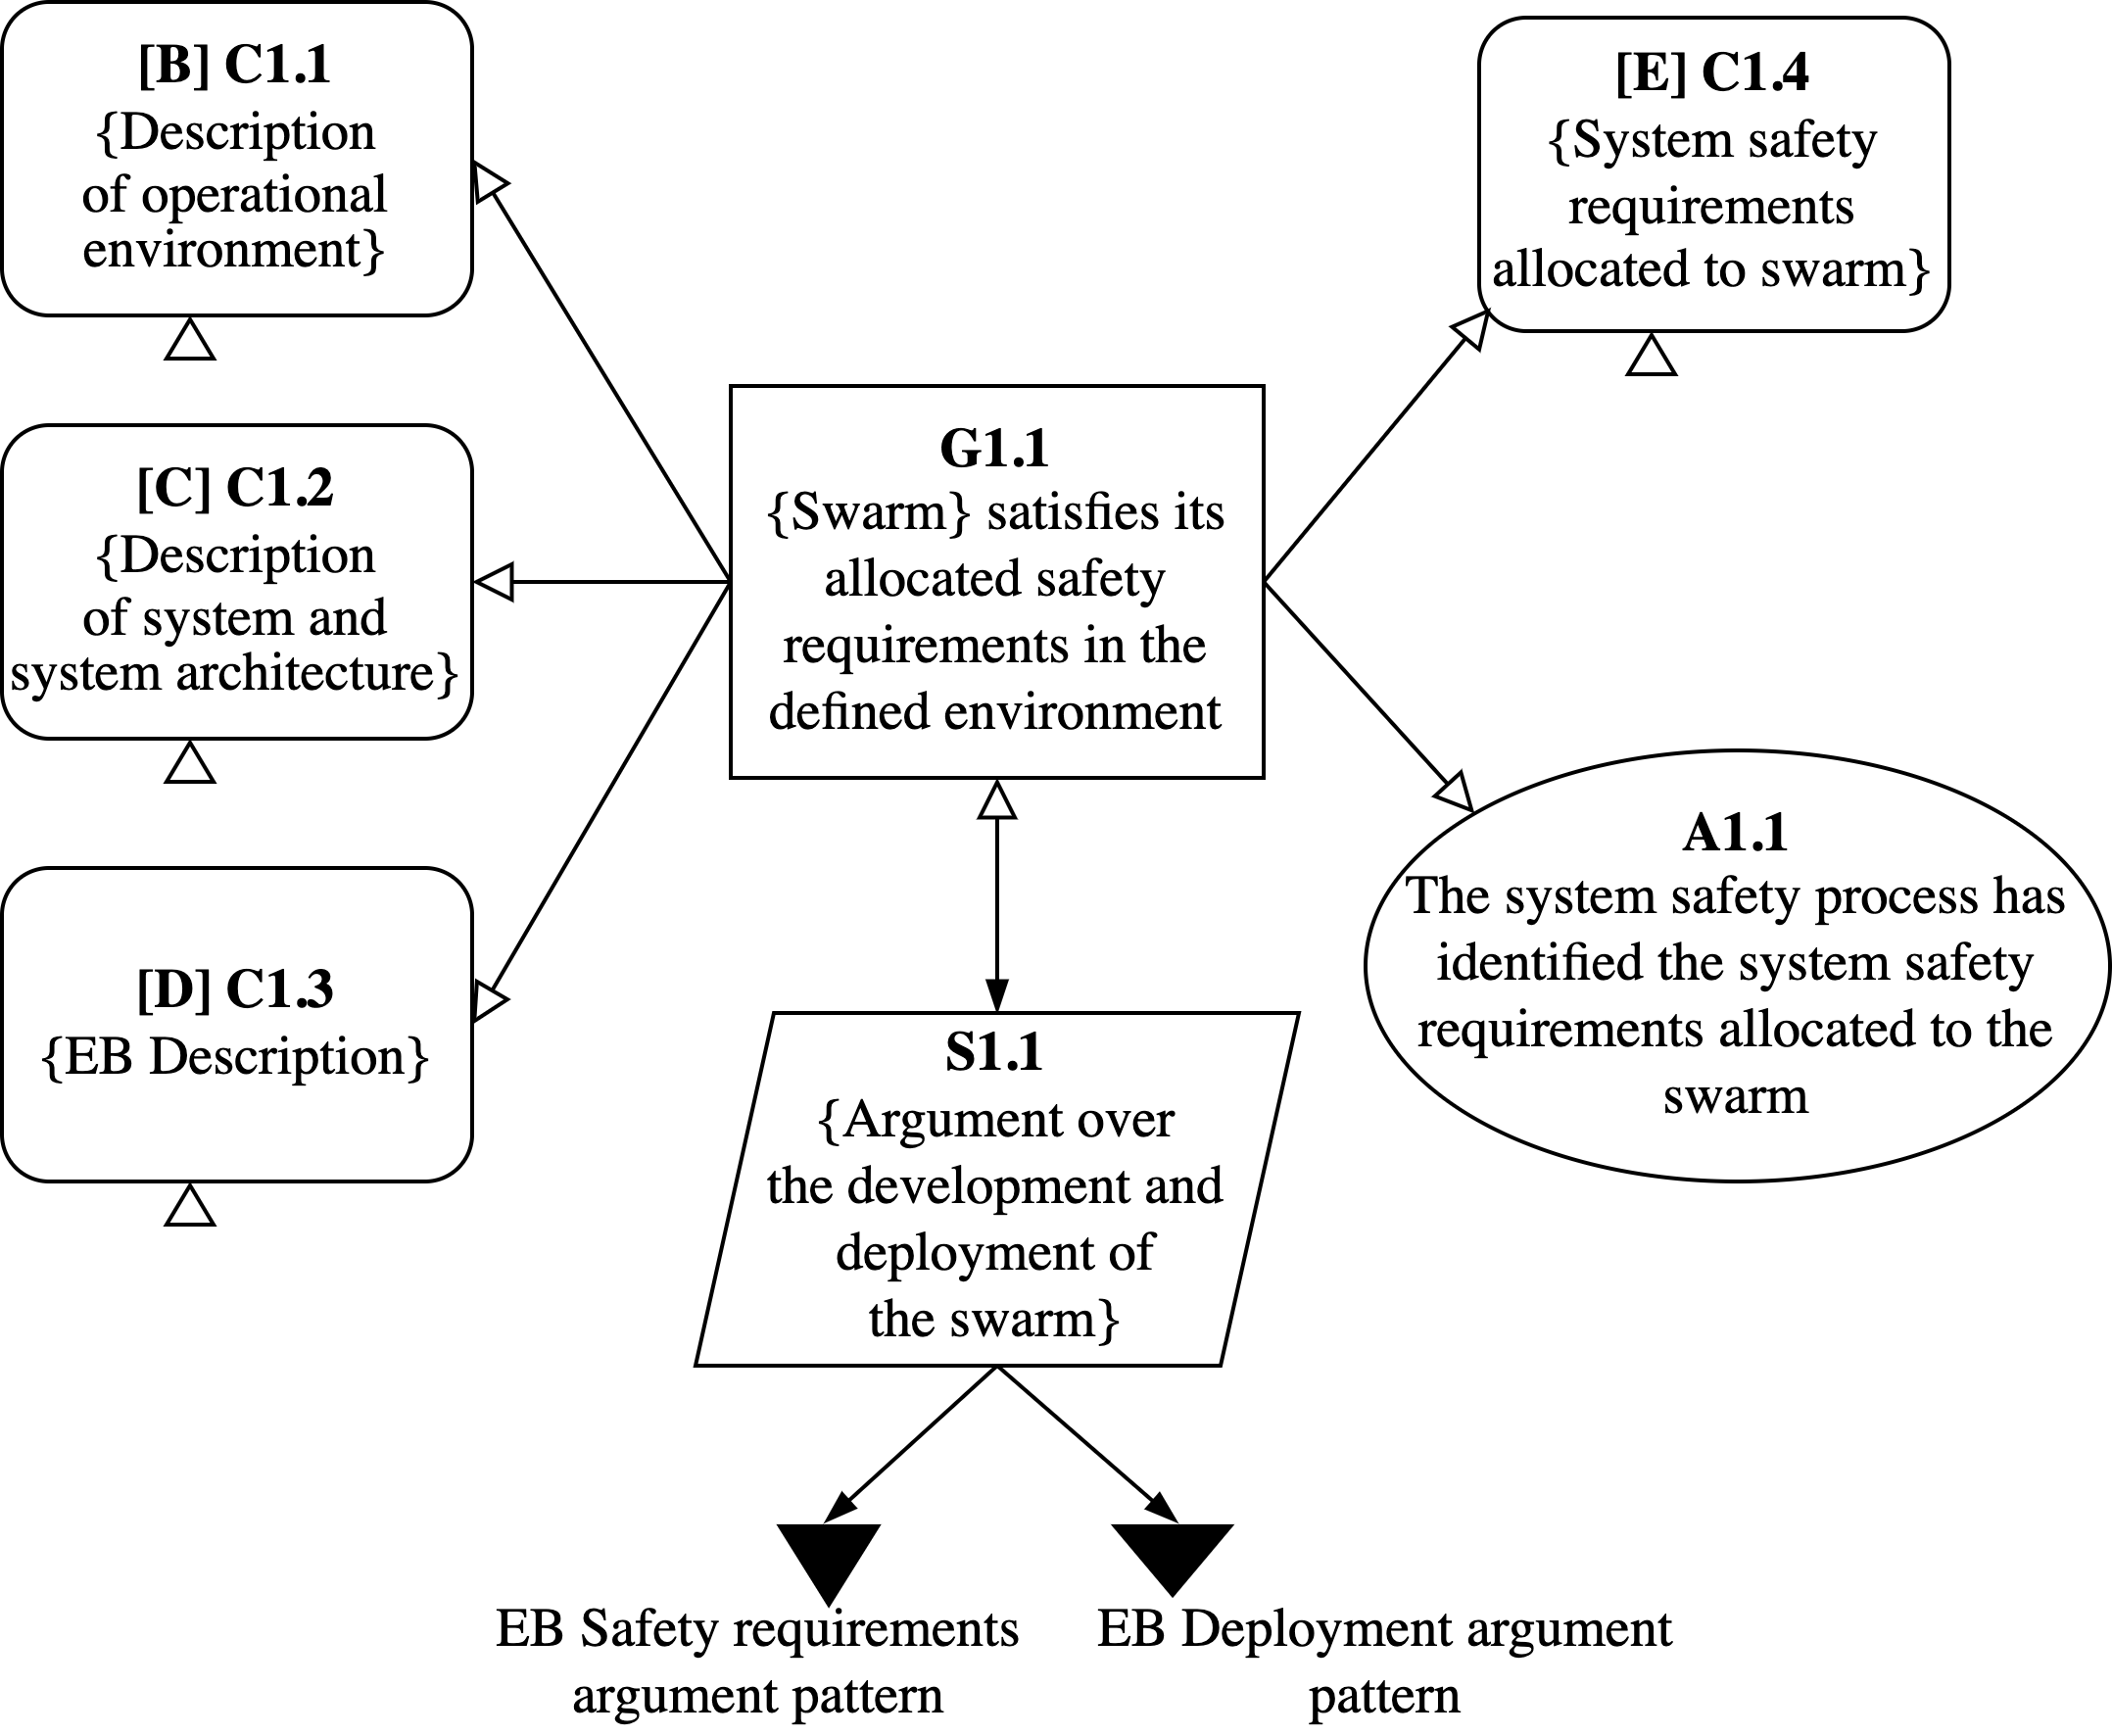
\includegraphics[width=0.4\textwidth]{figures/stage1-argumentpattern.png}
	\caption{EB Safety assurance scoping argument pattern.}
	\label{stage1-ap}
\end{figure}

\subsection{Stage 2: EB Safety Requirements Assurance} \label{framework-stage2}
%\noindent \textbf{\textit{[Lead:  WP1; Other: WP2, WP3]}}\\ 
%\noindent\textbf{\textit{[Author Guidelines: total 7 pages (maximum); \\Format/structure: Describe adapted AMLAS activities, inputs and outputs using cloakroom case study examples. \\
		%\noindent WP1 = (Activities: 3, 4, 5; Inputs: E, I; Outputs: H, J, K: 2700 words / 3 pages maximum))\\
		%\noindent WP2 = (List of Ethical Requirements and Description: 1800 words / 2 pages maximum)\\
		%\noindent WP3 = (List of Socio-Technical/Regulatory Requirements and Description: 1800 words / 2 pages maximum)]
		%}}\\
As in AMLAS, adapted Stage 2 contains three activities (Fig.~\ref{amlas-a-stage2}), which are performed to provide assurance in EB safety requirements for the swarm. 
In activity 5, the artefacts generated are used to instantiate the EB safety requirements assurance argument pattern. 
The scope of this stage is limited to the EB model of the swarm.\\

\begin{figure}[!t]
	\centering
	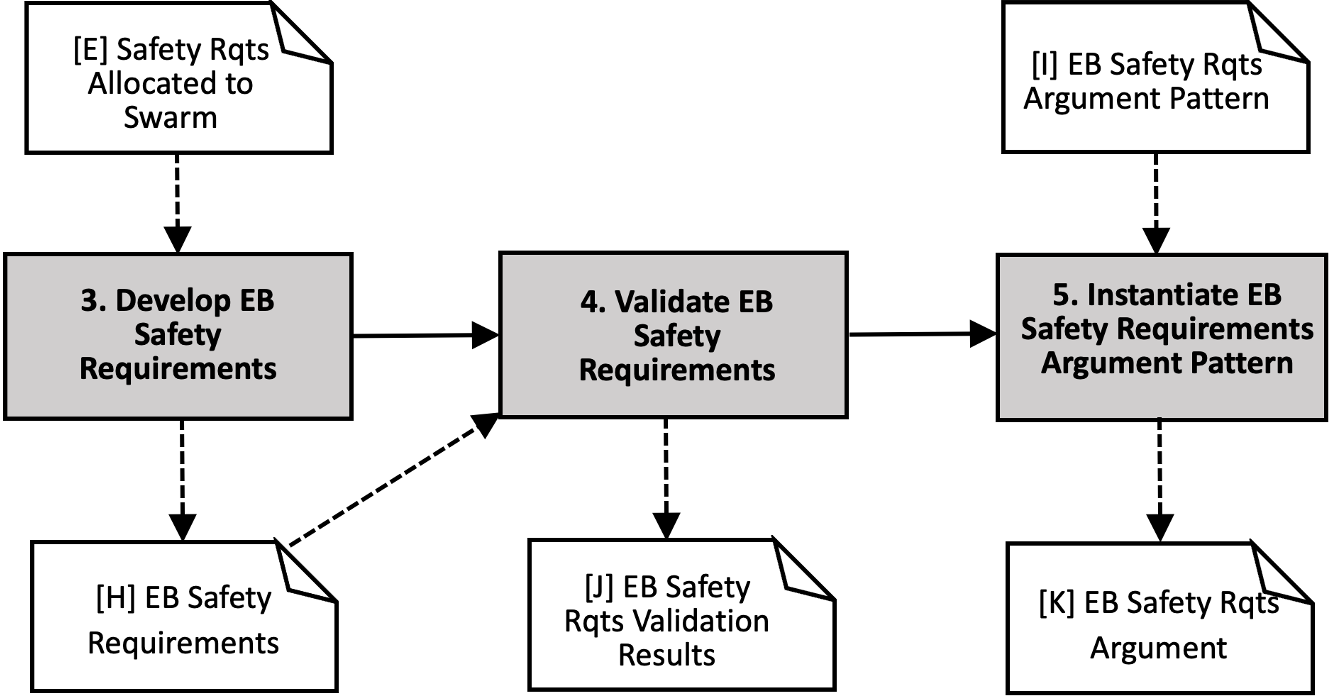
\includegraphics[width=0.5\textwidth]{figures/amlas-a-stage2-v2.png}
	\caption{Stage 2: Adapted AMLAS emergent behaviour safety requirements assurance process.}
	\label{amlas-a-stage2}
\end{figure}

\noindent \textbf{Activity 3: Develop EB safety requirements}

The required input to Activity 3 in Stage 2 is the safety requirements allocated to the swarm ([E]).
We define EB safety requirements to control the risk of the swarm to system-level hazards by taking into account of the defined system architecture and operating environment. 

As in AMLAS, although there can be a wide range of requirements for the swarm like scalability, security and interpretability, the EB safety requirements need to be limited to the ones that have an impact on the operational safety of the system. 
Other types of requirements (e.g. security, scalability) need to be defined as EB safety requirements, only if their behaviours or underlying constraints have an influence on the safety-criticality of the swarm's output.  

The AMLAS guidance prescribes two types of requirements for ML components: performance and robustness. 
In the swarm context, we consider four types of requirements: \emph{performance}, \emph{adaptability}, \emph{human safety}, and \emph{environment}.
Robustness in the swarm context is a more broad notion, thus we introduce adaptability and environment sub-categories. 
In AMLAS, one key approach when defining robustness requirements is to consider the dimensions of variation which exist in the input space. In the swarms context, this can be variation in the simulation space instead of the input space. 

We consider several performance safety metrics under the four requirements categories: 
(i) performance: low impact and high impact collisions; 
(ii) adaptability: percentage of swarm stationary outside of the delivery site, number of stationary agents, time since last agent moved; 
(iii) human-safety: velocity or average velocity of agents, swarm size, rate of human encountered, proximity to humans;
(iv) environment: sum of objects/$m^2$.

For the performance, adaptability and human-safety requirements categories, we formulate requirements under three sub-categories: \emph{faultless operations}, \emph{failure modes (graceful degradation)}, and \emph{worst case}. 
In the conventional AMLAS framework, the level of faults one expect in a single ML system is low. 
However, in a swarm system, we expect it to have more faults, as there are more agents which are more difficult to monitor. 
As for \emph{graceful degradation}, we mean what is the acceptable level of faults, their impact, and how the system should react when those faults are introduced. 
Thirdly, we consider requirements for \emph{worst case}, which account for the least acceptable impact the system should experience and means of avoiding it. \\

\noindent \textbf{Activity 4: Validate EB safety requirements}

The required input to Activity 4 in Stage 2 is the safety requirements allocated to the swarm ([E]). 
As suggested in AMLAS guidance, we use reviews and simulations to validate the EB safety requirements.\\

\textbf{Reviews:} the requirements derived for the cloakroom were also reviewed by a safety-critical systems engineering expert to ensure that the specified EB safety requirements for the swarm will deliver its intended safe operation. This expert has a wide experience in topics related to aerospace, defence and transportation; and safety of autonomous systems. Previously, this expert had reviewed the CovidSim modelling, which was instrumental in settling the UK lock-down policy. 

\textbf{Simulation: }We have validated several EB safety requirements (all performance, adaptability, and environment requirements except requirement RQ4.5) of the cloakroom system using a 3D simulator (Gazebo). This simulation is an exact replication of the 4m x 4m lab environment (see Fig.~\ref{3Dsim}). \\

\begin{figure}[!t]
	\centering
	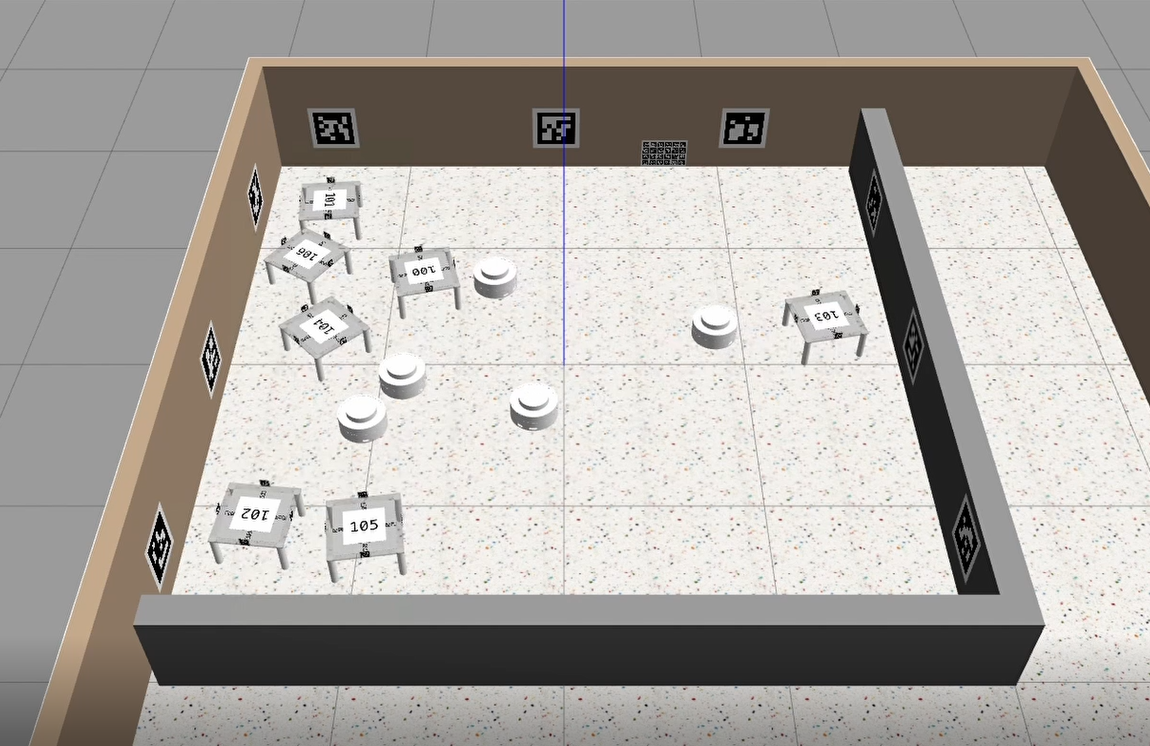
\includegraphics[width=0.5\textwidth]{figures/3Dsim.png}
	\caption{3D simulation created to validate several EB safety requirements of the cloakroom.}
	\label{3Dsim}
\end{figure}

\noindent \textbf{Stage 2 Requirements (Output H)}\\
\noindent \textbf{Cloakroom: Performance Requirements (see Table~\ref{tab:perormance}):}
\begin{table}[!t]
	\centering
	\begin{tabular}{|p{7mm}|p{72mm}|}
		\hline
		& \textbf{Requirements for Faultless Operations} \\
		\hline
		RQ1.1 & The swarm \emph{shall} experience \textbf{$<$ 1 low impact (V $<$ 0.5m/s)} collisions across \textbf{1000} seconds of faultless operation. \\ 
		\hline
		RQ1.2 & The swarm \emph{shall} experience \textbf{$<$ 1 high impact (V $>$ 0.5m/s)} collisions across \textbf{a day} of faultless operation. \\ 
		\hline
		& \textbf{Requirements for Failure Modes (Graceful Degradation): } \\
		\hline
		RQ1.3 & The swarm \emph{shall} experience \textbf{$<$ 10\%} increase in \textbf{low impact} collisions across \textbf{1000} seconds of operation with \textbf{10\% injection} of \textbf{full communication fault} to the swarm. \\
		\hline
		RQ1.4 & The swarm \emph{shall} experience \textbf{$<$ 0.1\%} increase in \textbf{high impact} collisions across \textbf{a days} operation with \textbf{10\% injection} of \textbf{full communication fault} to the swarm.\\ 
		\hline
		RQ1.5 & The swarm \emph{shall} experience \textbf{$<$ 10\%} increase in \textbf{low impact} collisions across \textbf{1000} seconds of operation with \textbf{50\% injection} of \textbf{half-of-wheels motor faults} to the swarm.\\
		\hline
		RQ1.6 & The swarm \emph{shall} experience \textbf{$<$ 0.1\%} increase in \textbf{high impact} collisions across \textbf{a days} operation with \textbf{50\% injection} of \textbf{half-of-wheels motor faults} to the swarm.	\\	
		\hline
		& \textbf{Requirements for Worst Case: } \\
		\hline
		RQ1.7 & The swarm \emph{shall} experience \textbf{$<$ 2 low impact (V $<$ 0.5m/s)} collisions across \textbf{1000} seconds of faulty operation. \\			\hline	
		RQ1.8 & The swarm \emph{shall} experience \textbf{$<$ 2 high impact (V $>$ 0.5m/s)} collisions across \textbf{a day} of faulty operation.  \\		[1ex] 		
		\hline
	\end{tabular}
	\caption{\label{tab:perormance}Performance requirements for the cloakroom.}
\end{table}    

\noindent \textbf{Cloakroom: Adaptability Requirements (see Table~\ref{tab:adaptability}):}
\begin{table}[!h]
	\centering
	\begin{tabular}{|p{7mm}|p{72mm}|}
		\hline
		& \textbf{Requirements for Faultless Operations} \\
		\hline
		RQ2.1 & The Swarm \emph{shall} have \textbf{$<$ 10\%} of its agents \textbf{stationary*} outside of the \textbf{delivery site} at a given time.
		*Assumption: Agents are considered stationary once they have not moved for $>$ 10 seconds.
		\\ 
		\hline
		RQ2.2 & All agents of the swarm \emph{shall} move at least every \textbf{100 seconds} if outside of the \textbf{delivery site}. \\ 
		\hline
		& \textbf{Requirements for Failure Modes (Graceful Degradation): } \\
		\hline
		RQ2.3 & The swarm \emph{shall} experience $<$ 10\% increase in \textbf{number of stationary agents} at any given time with 50\% injection of half-of-wheels motor faults to the swarm. \\
		\hline
		RQ2.4 & The swarm agents \emph{shall} experience $<$ 10\% increase in \textbf{stationary time} with 50\% injection of half-of-wheels motor faults to the swarm.\\ 
		\hline
		RQ2.5 & The swarm \emph{shall} experience $<$ 10\% increase in \textbf{number of stationary agents} at any given time \textbf{10\% injection} of \textbf{full communication fault} to the swarm.\\
		\hline
		RQ2.6 & The swarm agents \emph{shall} experience $<$ 10\% increase in \textbf{stationary time 10\% injection} of \textbf{full communication fault} to the swarm. \\	
		\hline
		& \textbf{Requirements for Worst Case: } \\
		\hline
		RQ2.7 & The Swarm \emph{shall} have \textbf{$<$ 20\%} of its agents \textbf{stationary*} outside of the \textbf{delivery site} at a given time.
		*Assumption: Agents are considered stationary once they have not moved for $>$ 10 seconds. \\			\hline	
		RQ2.8 & All agents of the swarm \emph{shall} move at least every \textbf{200 seconds} if outside of the \textbf{delivery site}.\\		[1ex] 		
		\hline
	\end{tabular}
	\caption{\label{tab:adaptability}Adaptability requirements for the cloakroom.}
\end{table}   
\noindent Metric: Swarm waiting time/time-in-area

\noindent \textbf{Cloakroom: Human Safety Requirements (see Table~\ref{tab:human-s}):}
\begin{table}[!h]
	\centering
	\begin{tabular}{|p{9mm}|p{72mm}|}
		\hline
		& \textbf{Requirements for Faultless Operations} \\
		\hline
		RQ3.1 & The agents in the swarm \emph{shall} travel at speeds of less than \textbf{0.5m/s} when within \textbf{2m} distance of a \textbf{trained human*.}
		\\ 
		\hline
		RQ3.2 & The agents in the swarm \emph{shall} travel at speeds of less than \textbf{0.25m/s} when within \textbf{3m} distance of a \textbf{member of the public}.
		\\ 
		\hline
		RQ3.3 & The agents in the swarm \emph{shall} only come within \textbf{2m} distance of a \textbf{human $<$ 10} times collectively across \textbf{1000 seconds} of \textbf{faultless} operations.
		\\ 
		\hline
		RQ3.4 & The swarm \emph{shall} only allow \textbf{$<$ 5 agents} to request intervention from a \textbf{trained human*} at a given time
		\\ 
		\hline
		RQ3.5 & A Trained human \emph{shall} monitor 5-20 agents at a given time.
		\\ 
		\hline
		RQ3.6 & The swarm \emph{shall} only allow \textbf{1 agent} to request input from a \textbf{member of the public} at a given time.
		\\ 
		\hline
		RQ3.7 & A member of the public \emph{shall} receive $<$ 5 agents of swarm information at a given time.
		\\ 
		\hline
		& \textbf{Requirements for Failure Modes: } \\
		\hline
		RQ3.8 & The swarm \emph{shall} experience \textbf{$<$ 10\%} increase in \textbf{human encounters} across 1000 seconds of operation with \textbf{10\% injection} of \textbf{full communication fault} to the swarm. \\
		\hline
		RQ3.9 & The swarm \emph{shall} experience \textbf{$<$ 10\%} increase in \textbf{human encounters }across 1000 seconds of operation with \textbf{50\% injection} of \textbf{half-of-wheels motor faults} to the swarm.\\ 
		\hline
		& \textbf{Requirements for Worst Case: } \\
		\hline
		RQ3.10 & The agents in the swarm \emph{shall} only come within \textbf{2m} distance of a \textbf{human $<$ 20} times collectively across \textbf{1000 seconds} of \textbf{faulty} operations.
		\\		[1ex] 		
		\hline
	\end{tabular}
	\caption{\label{tab:human-s}Human safety requirements for the cloakroom.}
\end{table}   
\noindent *Trained human in this case refers to workers within the case study setting. We assume that this individual has received relevant training \& experience in the use of the swarm system.\\

\noindent \textbf{Cloakroom: Environmental Specification (see Table~\ref{tab:environment}):}
\begin{table}[!h]
	\centering
	\begin{tabular}{|p{7mm}|p{72mm}|}
		\hline
		RQ4.1 & The swarm \emph{shall} perform as required in environmental density levels 0-4 \textbf{p$_o$* of objects (sum of boxes and agents)} in the environment.
		\\ 
		\hline
		RQ4.2 & The swarm \emph{shall} perform as required when floor incline is 0-20 degrees.
		\\ 
		\hline
		RQ4.3 & The swarm \emph{shall} perform as required in a dry environment.
		\\ 
		\hline
		RQ4.4 & The swarm \emph{shall} perform as required in smooth-floored environments with step increases no greater than 0.5cm.
		\\ 
		\hline
		RQ4.5 & The swarm \emph{shall} only operate in environments where humans have devices that identify the human’s whereabouts to the swarm agents.
		\\		[1ex] 		
		\hline
	\end{tabular}
	\caption{\label{tab:environment}Environment requirements for the cloakroom.}
\end{table}   
\noindent *p$_o$ = sum of objects  / m$^2$

\begin{table*}
	\centering
	\begin{tabular}{|l| l| l| l| l| l|} %{|*{18}{c|}}  % repeats {c|} 18 times 
		\hline
		\multicolumn{6}{|p{15cm}|}{\textbf{System: Cloakroom System} \newline \textbf{Specifier: Safety Engineer} \newline \textbf{Date: 03 October 2022} \newline The cloakroom system requires a high degree of transparency for the trained workers, but with less transparency for the customers, due to concerns of criminals exploiting it.} \\ \hline
		\multirow{2}{11cm}{\textbf{IEEE Std 7001-2021 subclause \newline (C = cumulative, NC = non cumulative)}} & \multicolumn{5}{c|}{\textbf{Levels}} \\ \cline{2-6}
		& 1 & 2 & 3 & 4 & 5 \\ \hline
		5.1.1 Users (NC) & $X^*$ & $X^*$ & & & \\ & $X^{**}$ & $X^{**}$ & $X^{**}$ & & \\ \hline
		\multicolumn{6}{|p{15cm}|}{Note- Two categories of users are defined as follows: \newline
			* \textit{Customers} who are non-expert users.\newline %Transparency is comparatively more important to this category compared to trained staff.
			** \textit{Trained staff} are expert or super users of the cloakroom. These can be deployers and administrators of the swarm, such as site managers. They require a medium level of understanding of how the swarm works, including the ability to ask an agent to explain its decisions, to predict the system's behaviour in a given situation and repair simple faults of agents.} \\  \hline
		5.1.2 General public and bystanders (NC) & X & X & & & \\ \hline
		\multicolumn{6}{|p{15cm}|}{NOTE—The individual robots in the swarm are clearly identified as robots, with warnings; they are fitted with cameras for navigation, with limited views so that they do not collect personal data. This group is only indirectly affected by the system. }\\ \hline
		5.2.1 Validation and certification agencies (C) & X & X & & & \\ \hline
		\multicolumn{6}{|p{15cm}|}{NOTE—Evidence of validation and certification to a lower degree is sufficient such as equipped with a data-logging system, given the less-sensitivity of the system.}\\ \hline
		5.2.2 Incident investigators (C) & X & X & & & \\ \hline
		\multicolumn{6}{|p{15cm}|}{NOTE—The cloakroom system must log all events securely to support incident investigations, noting that incident investigation may be triggered by a customer, or a watchdog raising concerns about the functions of the swarm. The agents in the swarm are equipped with a data logging system that records high level decisions (no personal data will be recorded). Levels 3--5 are not considered essential, as the agents in the swarm will only require a limited number of behaviours (with no learning).  }\\ \hline
		5.2.3 Expert advisors in administrative actions or litigation (NC) & X & & & & \\ \hline
		\multicolumn{6}{|p{15cm}|}{NOTE—The company should take into account ISO 9001 accreditation or equivalent for the swarm.}\\ \hline
	\end{tabular}
	\caption{\label{tab:transparency}System transparency specification for the cloakroom.}
\end{table*}

\subsubsection{System Transparency Specification for the Cloakroom}
In this section, we show how IEEE P7001 standard can be applied to specify transparency requirements for the Cloakroom prior to its implementation, which is known as a process of \textit{System Transparency Specification} (STS) \cite{IEEE-P7001}. IEEE P7001 describes a set of normative requirements on transparency and explainability, which must be satisfied to be labelled as compliant. % cite both

%\paragraph{System Transparency Specification for the Cloakroom}
A company that organizes bespoke events with 50 to 10000 attendees is looking to automate their cloakroom by deploying a swarm of robots to assist attendees (customers) to deposit, store and deliver their belongings (e.g. jackets) \cite{Jones2020}. % cloakroom paper 
%Mindful of the safety, operational and regulatory requirements of the healthcare sector
The system must prioritize public safety, and the company decides to use this standard on transparency as a draft specification for their engineers to more transparently communicate the decision-making processes of their automated cloakroom. %swarm system. 
The score sheet summarizing the outcomes of the assessment is shown in Table~\ref{tab:transparency}. \\

\subsubsection{Ethics Requirements}
Building on \cite{Porter2022}, and adapting it for our purposes, we developed ethics requirements for swarm robots around the ethical principles of beneficence, non-maleficence, respect for autonomy, and justice. We wrote a matrix outlining how each principle applies to each stakeholder (Tables  \ref{tab:beneficence}-\ref{tab:justice} in the appendices). To limit the scope of this paper, we decided to focus on the impact of our case study on members of the public, trained humans, manufacturers, and the company deploying the swarm, hence leaving aside questions about broader societal and environmental implications.

The main ethics requirements, each corresponding to a principle, are shown in Table \ref{tab:ethics} below. 
\begin{table}[!h]
	\centering
	\begin{tabular}{|p{9mm}|p{72mm}|}
		\hline
		& \textbf{ Ethics Requirements} \\
		\hline
		RQ1 & The swarm \textit{shall} provide benefits to stakeholders. \\ 
		\hline
		RQ2 & The swarm \textit{shall} avoid causing unjustified harm to stakeholders. \\ 
		\hline
		RQ3 & The swarm \textit{shall} avoid undue constraints on stakeholders' personal autonomy. \\
		\hline
		RQ4 & The swarm \textit{shall} allow fair treatment of stakeholders.  \\		[1ex] 		
		\hline
	\end{tabular}
	\caption{\label{tab:ethics}Ethics requirements for the cloakroom.}
\end{table}  

These broad requirements should be further specified, and this is where developing ethics matrices is helpful. The matrices allow us to identify benefits, risks of harm, and threats to autonomy and fair treatment caused by the development and deployment of the system. The significance and likelihood of the identified benefits, harms, and threats should then be considered to decide which can be tolerated and which should be addressed; for the latter, ethics sub-requirements should be developed to make changes to the design of the system, and so ensure the development of a more ethically aligned technology. Deciding which changes to prioritise is the most difficult part of the process, because there is no formulaic approach to follow; rather, this process requires interdisciplinary and multi-stakeholder discussions, individual and collective judgment, and ethics deliberation, which should include consideration of opportunity costs. However, that extends beyond the scope of this paper. Below we only give examples of how the matrices could be used to develop sub-requirements to specify RQ1-4. In line with the core aim of this paper, we only give examples focusing on the swarm's emergent behaviour.
\\
\paragraph{Beneficence requirements}
The principle of beneficence requires consideration of the benefits of the development and deployment of a system, and the stakeholders who will or may enjoy those benefits \cite{Porter2022}. It is contested to what extent the private sector should develop technologies that  benefit end users and other stakeholders, beyond merely avoiding harms (principle of non-maleficence). This is one of the limitations of applying ethical principles that have emerged from the healthcare setting, where professionals are expected to promote patients’ health and wellbeing, to a context where there is no professional duty to promote the interests of end users \cite{mittelstadt2019principles}. However, we believe it is important to consider the benefits a system may produce, and who the beneficiaries are, for three main reasons.

First, this requirement forces developers to reflect on the reasons why they are developing a certain technology in the first place, what societal impact they aim to achieve, and whether these are positive impacts. There is usually some form of benefit associated with technological innovation, and it is unlikely that a marketable system would provide no benefits to stakeholders other than the manufacturers themselves.However, if no  beneficial use of the system can be identified, this should immediately be taken as an indication that manufacturers should reconsider developing the technology, at least in its current form \cite{Qin}. Second, outlining potential benefits is a necessary step to determine whether, ultimately, these benefits will outweigh the potential harms posed by the technology. Third, manufacturers should reflect on who the beneficiaries are in order to assess how benefits and risks of harm are distributed across stakeholders.

Table \ref{tab:beneficence} illustrates the benefits a swarm system may produce in the cloakroom use case. To give one example, companies may benefit from the decentralised nature of the swarm, which is possible because swarm behaviour emerges from interactions across the individual agents. In particular, smaller businesses could benefit financially from the deployment of such a system. While bigger companies have the resources to invest in centralised robotic systems, which require dedicated heavy infrastructures and are designed to be optimised to meet the specific needs of the company, smaller businesses require fast, out-of-the-box setups that can easily adapt to different deployment scenarios. Thanks to their decentralised nature, robot swarms can offer this solution \cite{jones2020distributed}.
\\
\paragraph{Non-maleficence requirements}
The principle of non-maleficence requires consideration of how the development and deployment of a system may harm various stakeholders \cite{Porter2022}. The identification of risks of harm can, in turn, inform the development of design requirements to reduce the chance of harm eventuating. No system will ever be completely risk free, and discussions about what residual risks should be judged “acceptable” raises important ethical and legal questions that fall beyond the scope of this paper \cite{fraser2021residual}.

Table \ref{tab:maleficence} illustrates a wide range of harms that may derive from the development and deployment of a swarm robot in the cloakroom use case. In line with the traditional focus of safety assurance, the technical requirements discussed in this paper address the risks for physical harm; however, we agree with Porter and colleagues about the need to also consider  the non-physical harms machines may bring about \cite{Porter2022}. For example, end users in the cloakroom scenario may experience data privacy harms. This is because their personal data (e.g., names, email addresses, footages from cameras built on the robots) will be stored on the swarm agents and dispersed across agents in a decentralised manner, in the same way that other information is shared within the swarm. A core property of swarm robots is their robustness, which allows the swarm to continue performing its task, even when some of its agents are destroyed or have faults. Thus, it is possible to imagine scenarios in which the swarm would continue to operate even when one agent gets lost or breaks down whilst having a hard drive with people’s personal information onboard, thus posing risk of hard-to-discover data breach. In a small environment like the cloakroom use case that agent could be easily identified and quickly put in a restricted area for human operators to take care of it. However, this scenario would become more concerning if the swarm was deployed, for example, as a parcel delivery system in a university campus. Such a system would need to carry information about students’ names and addresses, as well as pictures of delivered packages, which may include frames with identifiable individuals or students’ doorsteps. In this much bigger, open, and dynamic environment, it is likely more difficult to identify and remove the agent. This example illustrates that a sub-requirement of RQ2 could require that users’ personal data are, by design, safely stored and shared across agents in the system, and safely destroyed in case of faulty agents.  
\\
\paragraph{Respect for autonomy requirements}
The principle of respect for autonomy forces us to consider how a system may interfere with humans’ capacity for self-governance or capacity to act according to their own’s considerations, desires, values, and motivations \cite{beauchamp2019principles}. Following \cite{Porter2022}, we focus on three dimensions of autonomy: (1) stakeholders’ ability to make personal choices, which requires that meaningful options are available to them; (2) informed consent, which requires that stakeholders are sufficiently informed about relevant facts or characteristics of the system; and (3) meaningful control, i.e. humans’ ability to stop or intervene in a system that is malfunctioning, and ensure that it is acting as intended and desired.

Table \ref{tab:autonomy} illustrates the ways in which the development and deployment of a swarm robot in the cloakroom scenario may constrain stakeholders’ autonomy in these three dimensions. For example, the emergent behaviour of the system could interfere with business policies in a way that constrains operators’ options. We could imagine a scenario in which the unpredictability that characterises swarms’ emergent behaviour causes a human operator to violate their company’s health and safety policy that prohibits them to step over a robot or walk in an area where there is high density of agents, in an attempt to avoid personal injury or remove a faulty agent. This suggests RQ3 needs to be further specified to require that business policy and system requirements are consistent with each other.

The condition of informed consent would require end users to be informed about system functioning and capability, potentially including information about the swarm’s emergent behaviour. However, translating this condition into a sub-requirement of RQ3 raises challenging questions about the extent and depth of information that end users need. While transparency is often listed among the principles needed for the adoption of socially beneficial systems \cite{IEEEAligned}, we agree with others that it should not be considered an end in itself \cite{Porter2022}. Increased transparency leads to the desired outcome (in this case, opportunity for informed consent) only if what is made transparent is understandable to end users \cite{ananny2018seeing}. Thus, we should aim for decreased opacity, by providing relevant information to end users, tailored to their level of understanding and the role they play in the use case space, so that system behaviour becomes explainable to non-experts. The IEEE Standards Association has recently published a new standard on transparency of autonomous systems, to which we referred above \cite{IEEETransparency}.

Finally, the autonomy matrix highlights important challenges to attribution of responsibility. Moral responsibility refers to what makes a moral agent praiseworthy or blameworthy for some outcome, and differs from legal responsibility, which usually carries an enforceable obligation to redress the harm caused \cite{burton2020mind}. Moral responsibility usually requires two conditions: knowledge and control \cite{santoni2021four}. A swarm that adapts through emergent behaviour generates a “responsibility gap” \cite{matthias2004responsibility}, i.e. it makes it difficult to attribute responsibility for any harm caused, because the conditions may not be met for developers to give valid consent to system deployment nor to have meaningful control over the system once deployed. Because the emergent behaviour is not explicitly written, developers may not have an understanding of the inner decision-making of the swarm as a whole, and so the swarm’s emergent behaviour may depart from their intentions, leading to unwanted behaviour. To address this gap, a sub-requirement of RQ3 could require that the system uses a human readable controller (e.g., decision trees), which allows humans to explain it, analyse it for insight, and make improvements to system performance, hence conferring some level of understanding and control back to developers \cite{jones2019onboard}. Moreover, developers could be required to use the framework described in this paper to develop system specifications, given that assurance of swarm’s emergent behaviour is the core aim of the present work. 
\\
\paragraph{Justice requirements}
The principle of justice requires us to treat others in a fair, equitable, and appropriate way in light of what is due or owed to them \cite{beauchamp2019principles}. Among the main understandings of the concept, \textit{distributive justice} refers to the equitable and appropriate distribution of benefits and burdens, and so differs from \textit{procedural justice}, which focuses not on the fairness of the final allocation but of the procedures used to determine the allocation. \textit{Corrective justice} aims to rectify the injustice that one person has inflicted over another, and requires the existence of mechanisms for redress to be enacted \cite{sep-justice}. In contrast, \textit{retributive justice} is about inflicting punishment to those who have committed certain kinds of wrongful acts (e.g., negligence) \cite{sep-justice-retributive}. 

In Table \ref{tab:justice}, we used these different understandings to distil the ways in which the development and deployment of the swarm may cause unfair treatment of various stakeholders in the cloakroom use case \cite{Porter2022}. The threat to justice that more clearly relates to swarms’ emergent behaviour concerns the procedure in which objects are deposited and retrieved. For example, a robotic cloakroom may lead to unfair treatment of people who are arguably entitled to retrieve their belongings first based on need, such as people who have deposited their mobility aids together with their jackets. In a cloakroom implementation in which the swarm agents move around the area by performing random walks, which are easy to implement with no centralised control unit \cite{jones2020distributed}, there is no priority order. When an agent finds a box that has been requested, it brings it back, even if it happens that that box was ordered later than another box.

This may be unproblematic in a small cloakroom, where waiting times are usually short. In a bigger area, a sub-requirement for RQ4 could be introduced to establish a priority mechanism for “priority items” like mobility aids. However, care should be exercised in the implementation of this requirement. If agents started to ignore other items until they found and retrieved priority objects, it would likely reduce swarm efficiency. As a minimum, this would require stakeholders to make difficult decisions about how to strike a balance between efficiency and fairness; a significant decrease in system efficiency would end up disadvantaging those whose needs we want to prioritise. A better solution to implement a priority requirement would be to make it more likely that swarm agents carry boxes with priority items and so are ready to deliver them upon user’s request. This could be achieved by leveraging on other properties that a robot swarm needs by design, like reshuffling, where agents are designed with a probability to pick up a box they encounter and move it for a limited time, even if it is not of their interest \cite{milner2022stochastic}. Reshuffling is necessary in use cases like the cloakroom to avoid occluded boxes in the centre of a pile never being found. The probability of picking up and dropping a box may be changed so that agents encountering a priority item are required to carry it around for a little longer, hence increasing the chances that they will have it when that item is requested back. This example illustrates that, even when ethics requirements are clear, judgment still needs to be exercised in how to best implement them in a specific use case.  
\subsubsection

% BEGINING OF PETE'S ADDITION

\subsubsection{Using the Structural, Organisational, Technological, Epistemic, and Cultural (SOTEC) framework for a regulatory requirements analysis of autonomous robotic swarms}

This section outlines Macrae’s \cite{macrae2021learning} Structural, Organisational, Technological, Epistemic, and Cultural (SOTEC) framework of sociotechnical risk in Autonomous and Intelligent systems (AIS) and discusses its regulatory implications for autonomous swarms in a cloakroom scenario. The SOTEC framework proposes that risk and failure in AIS be understood in terms of five broad sociotechnical categories, each corresponding to different organisational, contextual, and human factors that might inform AIS safety requirements. The spotlight on sociotechnical sources of risk in AIS throughout section one provides a crucial launching point for the identification of regulatory requirements. Viewing regulatory requirement analysis from a sociotechnical perspective allows us to move away from a purely technical conception of requirements, and helps us design autonomous systems that better fit the organisation and operators’ work in which safety considerations are meaningful within the wider system and operational context. Based on these considerations, we illustrate the relevance of the SOTEC framework for crafting regulatory requirements for autonomous robotic swarms as a safety assurance mechanism. Following this, we then apply the framework by utilising insights from swarm engineers who are in the process of developing a case study of a swarm system for a cloakroom setting that is in early development and offering autonomous solutions to customers depositing their garments.

\paragraph*{The relevance of the SOTEC framework for regulatory requirements}

Most pre-existing work on safety assurance in AIS has focused on developing technical aspects of assurance \cite{brundage2020toward}. The work has proven challenging (e.g. \cite{karvonen2020safety}, \cite{thieme2021proceedings}, \cite{sanchezexplainable}). The causes of some highly visible AIS failures were unforeseen, and therefore untested and unmanaged. The latent problem with Uber’s self-driving computer vision system, which led to the first autonomous vehicle

% TODO: WEBPAGE - CITE LATER

fatality in 2018 (Niedermeyer, 2019), is one example. We might also look to the `object classification’ failures in the STM Kargu-2 lethal autonomous weapons system, which may have led it to hunt down and remotely engage retreating Libyan soldiers in March 2020 \cite{nasu2021kargu} or to a fault in an AI designed for diagnosing skin cancer, which misled clinical experts in 2019 \cite{tschandl2020human}.

Such failures have eluded experts because their causes are rarely reducible to technical criteria alone. There is always a degree to which those causes lie in the wider `sociotechnical’ dimensions of autonomous and intelligent systems: the fact that AIS are “… designed, developed, built, deployed, maintained, supervised, operated, and governed by people,” as Macrae \cite{macrae2021learning} puts it, and that those people operate within complex social, cultural, and organisational processes” (see also: \cite{pettersen2021organizational}, \cite{reason2016managing}). So it is, Macrae \cite{macrae2021learning} argues, that researchers developing assurance tools for autonomous systems should consider sociotechnical sources of risk and failure, and illustrates five intersecting dimensions along which such risks might be understood. He labels these: Structural; Organizational; Technological; Epistemic, and Cultural (‘SOTEC’). Each category is outlined briefly below and  analysed in terms of the swarm context.

\paragraph*{Application of the SOTEC framework for regulatory requirements}
\textbf{Structural} sources of risk arise from the way different human and nonhuman elements in a system interact, allowing failures in one area to rapidly degrade or impact on other parts of the system. For example, a fault in the upwards facing camera on a single swarm agent may allow a minor disruption – a person removing the box – to quickly amplify and grow into a situation where the agent is unable to detect whether the human has removed the box. Here, the fault in the structural character of the camera brings to light the risk of a swarm agent continuing to think that it is carrying the box and as a result it stops searching (whereas it should be searching or executing another task). This disruption in one part of the system then effects the broader context of the swarm system not only by reducing the overall optimal efficiency of the swarm (especially if the agent is trying to compete with other agents) but also because of the potential to grow into a critical situation where other agents are likely to give the faulty agent preference in hallways or corridors, potentially cluttering up the environment members of the public are permitted to move in. 

Macrae \cite{macrae2021learning} might call this type of structural failure in a swarm context a “disruption amplifier”.  As a result, disruption amplifiers are tied to the production of a particular and specific regulatory requirement; namely, the project of engineering the identification and prevention of disruption amplifiers, in the form of swarm engineers developing a system that can identify features which cause disruptions or failures and preventing these from enlarging, expanding, or developing into more critical situations which are harder to deal with or recover from. For swarm researchers interested in this type of project, a way of doing it might be to have all the other agents in the swarm (using their functioning radial camera) expressing to the agent (which has the faulty camera) to stop thinking that there is still a box on its head. In a broader perspective, one could also include other diverse regulatory requirements such as `identification and prevention of failure cascades’, `state of vigilance’, and `creation of test permeabilities’, as detailed in the Appendices. However, as our focus in on disruption amplifiers, the regulatory requirements that we are concerned with here are those that are directly tied to preventing system features which cause disruptions or failures to enlarge. 

\textbf{Organizational} sources of risk emerge when organizational structures — such as rules and expectations — are insensitive to the vagaries of real human behavior and ineffective at detecting and managing errors. For example, if a swarm agent is on its own and away from the rest of the swarm and has a significant error, yet there is no alerting process in place to inform human operators that the agent has the error, it is unlikely that the operators will ever see the error message. This means that there is no system in place to issue alerts regarding the status and activities of the faulty individual agent that has gone, for want of a better word, `rogue’. Although the swarm may be able to continue to perform efficiently without the rogue agent, serious safety incidents could take place without going noticed (for instance, if a fault with the agent’s obstacle avoidance system is not detected the agent has the potential to bump into people’s shins. Macrae \cite{macrae2021learning} might call this type of organizational failure in a swarm context ``invisible automation”. As a result, invisible automation is tied to the production of a particular and specific regulatory requirement; namely, the project of engineering translucency around error reporting, in the form of the organization creating organizational processes that are effective at detecting and managing errors. For instance, ensuring that each agent is fitted with lights that flash red in order to draw operator attention. In a broader perspective, one could also include other diverse regulatory requirements such as `safety expertise and leadership’, `supervision’, `regulative mechanisms’, and `access to governance and standards', as detailed in the Appendices. However, as our focus is on invisible automation, the regulatory requirements that we are concerned with here are those that are directly tied to the existence of alerting processes to not only inform swarm operators that the agent has an error or fault, but also to manage it.

\textbf{Technological} sources of risk arise from the specific capabilities and constraints inscribed into and produced by the system itself. For example, if the swarm agents are made to have limited memory, recorded pieces of important information are unlikely to reach the operator in time to prevent a hazard. This is especially the case, when from a sociotechnical perspective, engineers produce individual agents that have limited memories so that when the agent detects or records a hazard (for example, a dropped garment) information about the hazard is deleted or overwritten by new information and that critical information about the hazard gets lost. Considered in this way, building swarm agents with a limited memory (say, that only retain information for 10 seconds before it gets overwritten or deleted) stops critical information about hazards or risks reaching the operators who are able to prevent accidents from happening. 

Macrae \cite{macrae2021learning} might call this type of technological risk in a swarm context “hazard masking”. As a result, hazard masking is tied to the production of a particular and specific regulatory requirement; namely, the project of engineering the non-masking of hazards, in the form of engineers building technical processes or features that do not inadvertently hide, disguise, or render ambiguous information. For instance, ensuring that agents are not built with limited memory and the system does not delete or overwrite information, or that the system has some form of distributed method in place so that information can be effectively distributed across the swarm generating a ``collective memory” \cite{wilson2022information}. In a broader perspective, one could also include other diverse regulatory requirements such as `open capability’, `automation maturity’, and `no self-reliance on internal infrastructure’, as detailed in the Appendices. However, as our focus in on hazard masking, the regulatory requirements that we are concerned with here are those that are directly tied to the existence of technical processes, components or features that have been designed to inadvertently hide, disguise, or render ambiguous hazards.

\textbf{Epistemic} sources of risk arise from the ways that human knowledge is often incomplete, wrong, or out of date: creating pockets of ignorance that hide unexpected hazards. For example, if the swarm system has been tested in a software simulation but not in a real-world environment outside of controlled laboratory conditions, it is likely to fall whim to a lack of sufficient knowledge about the limits of the system prior to its deployment in the real world. This might be the case where the engineer has confidently calculated the maximum range of the lidar detection sensor in the 3D simulation, but fails to take into consideration the `reality gap’ of what this maximum range might look like in a real world hardware example. The seeming difficulty of not preparing for a nonlinear response from the hardware in the real world (as opposed to a linear response in the safe world of the simulation test) means that a retuning sensor value of 0.5 which may trigger a 30 centimeter avoidance movement in the simulation might mean something different in the real world. Because the engineer has not tested this 0.5 in the real-world, the 30 centimeter avoidance might turn into 10 centimeters. Because of this, the engineer believes they have built a good avoidance system in simulation and testing when, in fact, the agent in the real world is returning a value which is imprecise and does not provide enough of a stopping distance to prevent a collision. 

We call this type of epistemic risk in a swarm context `insufficient testing’ and may also be thought as a type of ``simulatory inattention” \cite{macrae2021learning}, however, our definition differs from Macrae in that testing must also be conducted outside simulation software and into the real world with hardware outside the laboratory environment. As a result, insufficient testing is tied to the production of a particular and specific regulatory requirement; namely, the project of engineers conducting `sufficient testing', in the form of producing knowledge about tests that is not partial, incorrect, or out of data and stopping pockets of ignorance to develop. For instance, ensuring that the testing of software and hardware is a central part of the swarm development and testing program, with swarm developers ensuring that there are no incompatibilities between softwares AND between software and hardware. In a broader perspective, one could also include other diverse regulatory requirements such as `leading the learning', `operational engagement’, `sensitivity to experience’, and `transparent, cooperative and open safety’, as detailed in the Appendices. However, as our focus in on insufficient testing, the regulatory requirements that we are concerned with here are those that are directly tied to a programme of testing for every level of resolution that is available to the engineer before the swarm is deployed, including the final physical system and hardware outside of controlled lab conditions. 

\textbf{Cultural} sources of risk arise from collective values, beliefs, norms and practices, which surround and inevitably shape AIS design and operation. For example, if there is a poor cultural pattern of communication that discourages or makes it difficult for swarm engineers to coordinate with each other on different aspects of system development there may be pauses or gaps in understanding how failures emerge and are interpreted. This could manifest on many levels, such as individual, team, and society levels. On a team level, for example, there could be an awareness of a faulty algorithm or problem that the team wishes to solve but may not communicate this to the other team for sake of meeting ambitious targets linked to academic pressure to publish. Similarly, if a team of swarm operators have not yet developed a pipeline through which performance data is not regularly updated and distributed across the development chain, then opportunities to improve the system will fall short because those issues that are occurring in reality are unlikely to be resolved. 

Macrae \cite{macrae2021learning} might call this type of cultural risk in a swarm context “developmental disintegration”. As a result, developmental disintegration is tied to the production of a particular and specific regulatory requirement; namely, the project of `merging development activities’, in the form of operators ensuring that there is ongoing and transparent coordination between the multiple teams involved in different testing activities. For instance, creating a culture that privileges the rapid and wide distribution of simulation and real world data, and prioritizes safety oversight and assurance. In a broader perspective, one could also include other diverse regulatory requirements such as `definitive reliability’, `encouraging operators to raise concerns and question decisions’, `removing existential pressure’, and `ongoing monitoring, recording and reporting of real metrics and their properties’, as detailed in the Appendices. However, as our focus in on developmental disintegration, the regulatory requirements that we are concerned with here are those that encourage corporate values and norms that emphasise the importance of integrated, proactive and centralised risk management.

The SOTEC framework is a relatively blunt instrument, but offers a useful tool for stimulating awareness and discussion of non-technical issues in requirements engineering. In the context of robotic swarms, for example, it encourages critical reflection on the constraints of their operational environment, and on the needs and expectations of the people with whom they will interact. Most generally, it highlights a range of `sociotechnical’ risks that could be useful in framing regulatory requirements for autonomous systems. However, at this early stage, what follows is meant merely to be suggestive, and this will continue until we start observing the work of potential users (such as human operators and members of the public). In this way, our work isn’t too dissimilar to traditional requirements engineering because it draws on the authors’ underlying assumptions of social and technical behaviour through which the swarm may operate in a cloakroom scenario. Such limitations can in fact be overcome if we acknowledge that future research needs to explore these requirements in depth and contingent on the involvement of humans using the system, for instance. Nevertheless, this article uses Macrae’s SOTEC framework \cite{macrae2021learning} as a starting point for a theoretical conceptualisation of swarm-human risks and regulatory requirements. Please see the appendices where we present the risks within a cloakroom context, and identify regulatory requirements on the basis of that setting.


% END OF PETE'S ADDITIONS

\subsection{Stage 3: Data Management} \label{framework-stage3}
% \noindent \textbf{\textit{[Lead:  WP5]}}\\ 
% \noindent\textbf{\textit{Author Guidelines: 900–1800 words / 1–2 pages (maximum); \\Format/structure: Describe adapted AMLAS activities, inputs and outputs using cloakroom case study examples. Activities: 6, 7, 8; Inputs: H; Outputs: L0, L1, M, N, O, P, Q, S}}\\
% See Fig.~\ref{amlas-a-stage3}
% \begin{figure*}
% 	\centering
% 	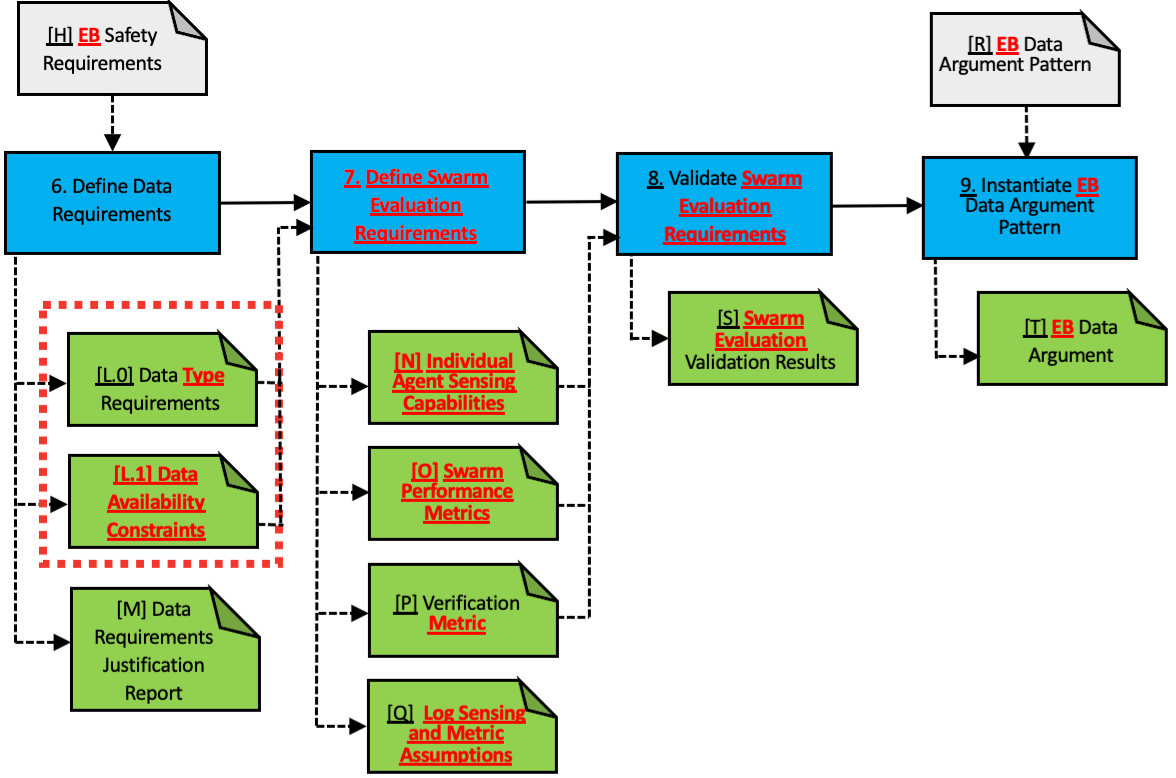
\includegraphics[width=1.0\textwidth]{figures/amlas-a-stage3.png}
% 	\caption{Adapted AMLAS data management process.}
% 	\label{amlas-a-stage3}
% \end{figure*}

In the case of designing emergent behaviours data plays a vital role, though one that differs from the machine learning applications AMLAS was initially designed for. In order to address this difference, the following activities and outputs have been adjusted to take into account the swarm behavioural design process and the added complexities that come with multiple agents interacting with one another.

\begin{figure*}
	\centering
	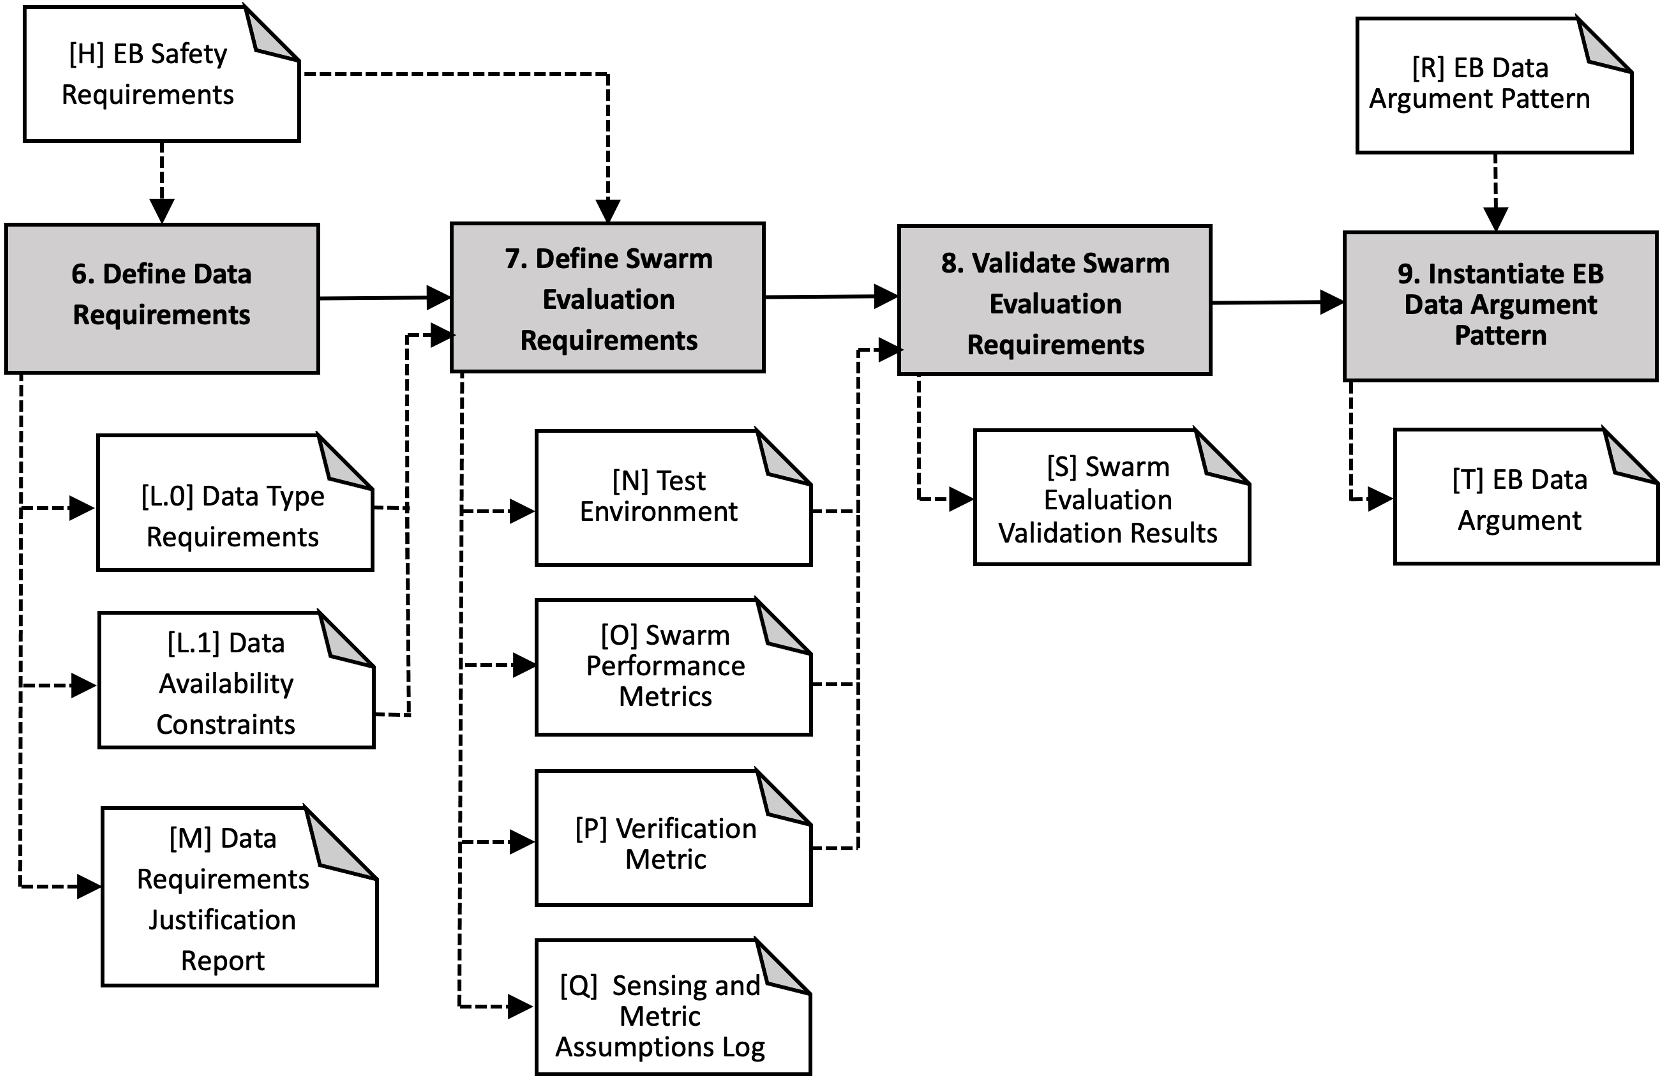
\includegraphics[width=0.8\textwidth]{figures/Stage3_DM_V2.png}
	\caption{Adapted AMLAS data management process.}
	\label{amlas-a-stage3}
\end{figure*}

\subsubsection*{Activity 6. Define Data Requirements}

% AMLAS - This activity requires as input the ML safety requirements ([H]) as described in Stage 2 and, from these requirements, data requirements ([L]) shall be generated. Of particular interest in the development of data requirements are those safety requirements which pertain to the description of the system environment.

In our adaptation of activity 6 we take the emergent behaviour safety requirements [H] outlined in Stage 2 as an input. These safety requirements guide the data requirements in this activity, feeding into the data specification that we outline here. Unlike the original AMLAS framework, we have split the data requirement [L] into two multi-agent focused requirements: [L.0] data type requirements and [L.1] data availability constraints.

\paragraph*{[L.0] Data Type Requirements}

This elements focus on the relevance, completeness, accuracy, and balance of the information that will be used to construct the swarm behaviour and will be subsequently used to test the emergent behaviour of the system prior to its deployment.

The relevance of the data used in the development of the emergent behaviour specifies the extent to which the test environment must match the intended operating domain into which the model is to be deployed. Examples of requirements relating to relevance are shown in Table \ref{tab:L0_relevance}.

\begin{table}[h]
    \centering
    \begin{tabular}{p{1cm} p{6cm}}
        \textbf{ID} & \textbf{Example} \\
        \hline
        RQ 5.1 & All simulations shall include environments with different ranges of incline between 0-20\textdegree.\\
        \hline
        RQ 5.2 & All simulations shall be conducted in a dry environment.\\
        \hline
        RQ 5.3 & All simulations shall include floors with step increases that are $\leq$ 0.5 cm.\\
    \end{tabular}
    \caption{Relevance requirement examples for output [L.0].}
    \label{tab:L0_relevance}
\end{table}

The completeness of the data specifies the conditions under which we test the behaviour algorithm i.e. the volume of experiments or tests that will be run, the variety of tests executed, and the diversity of environments expected to be used in the testing process. Requirements examples relating to completeness are shown in Table \ref{tab:L0_completeness}.

\begin{table}[h]
    \centering
    \begin{tabular}{p{1cm} p{6cm}}
        \textbf{ID} & \textbf{Example} \\
        \hline
        RQ 6.1 & All simulations shall be repeated to include fault injections representative of full communication faults.\\
        \hline
        RQ 6.2 & All simulations shall be repeated a sufficient number of times to ensure results are representative of typical use.\\
        \hline
        RQ 6.3 & All simulations shall be repeated in multiple environments representative of those expected in real-world use of the system.\\
        \hline
        RQ 6.4 & All simulations shall include sufficient range of robot density levels within the scope of the operational domain.\\ 
    \end{tabular}
    \caption{Completeness requirement examples for output [L.0].}
    \label{tab:L0_completeness}
\end{table}

Accuracy in this context relates to the parameters defining the performance of the swarm systems primary function. For example, what constitutes a delivery in a logistics scenario, or under what conditions would an area be considered explored in a surveying mission. Table \ref{tab:L0_accuracy} shows some data requirement examples relating to accuracy.

\begin{table}[h]
    \centering
    \begin{tabular}{p{1cm} p{6cm}}
        \textbf{ID} & \textbf{Example} \\
        \hline
        RQ 7.1 & All boxes shall only be considered `delivered’, if all four of the boxes’ feet are positioned within the delivery zone.\\
        \hline
        RQ 7.2 & All boxes shall only be considered `delivered’, once they are no longer in direct contact with a swarm agent.\\
    \end{tabular}
    \caption{Accuracy requirement examples for output [L.0].}
    \label{tab:L0_accuracy}
\end{table}

Balance, outside of a machine learning use case, refers the balance of the trials executed in the testing process of the emergent behaviour algorithm. By considering balance, we expect the number of tests conducted for individual failure modes or environment types to be justified, ensuring that there is not an unrealistic bias in testing towards a particular scenario. Some examples of data requirements relating to balance are listed in \ref{tab:L0_balance}.

\begin{table}[h]
    \centering
    \begin{tabular}{p{1cm} p{6cm}}
        \textbf{ID} & \textbf{Example} \\
        \hline
        RQ 8.1 & All simulations shall be repeated so as to obtain representative evaluations for each possible mode of failure (defined under performance, adaptability and human-safety requirements in Stage 2).\\
        \hline
        RQ 8.2 & All simulations shall be repeated equally across all test environments.\\
        \hline
    \end{tabular}
    \caption{Balance requirement examples for output [L.0].}
    \label{tab:L0_balance}
\end{table}

%In Table \ref{tab:L0} we list each of the requirement focuses considered in this output and provide respective examples of swarm data requirements.

% \begin{table}[H]
%     \centering
%     \begin{tabular}{p{2cm} p{6cm}}
%         \textbf{Requirement} & \textbf{Example} \\
%         \hline
%         Relevance & All simulations shall include environments with different ranges of incline between 0-20\textdegree.\\
%         \hline
%         & All simulations shall be conducted in a dry environment.\\
%         \hline
%         & All simulations shall include floors with step increases that are \leq 0.5 cm.\\
%         \hline
%         Completeness & All simulations shall be repeated to include fault injections representative of full communication faults.\\
%         \hline
%         & All simulations shall be repeated a sufficient number of times to ensure results are representative of typical use.\\
%         \hline
%         & All simulations shall be repeated in multiple environments representative of those expected in real-world use of the system.\\
%         \hline
%         & All simulations shall include sufficient range of robot density levels within the scope of the operational domain.\\
%         \hline
%         Accuracy & All boxes shall only be considered `delivered’, if all four of the boxes’ feet are positioned within the delivery zone.\\
%         \hline
%         & All boxes shall only be considered `delivered’, once they are no longer in direct contact with a swarm agent.\\
%         \hline
%         Balance & All simulations shall be repeated equally across all test environments.\\
%         \hline
%         & All simulations shall be repeated equally across all test environments.\\
%     \end{tabular}
%     \caption{Requirement focuses for output [L.0] with representative examples from the cloakroom use case.}
%     \label{tab:L0}
% \end{table}

\paragraph*{[L.1] Data Availability Constraints}

With the introduction of multiple agents comes the issue of data availability. Distributed communication is a key feature found in emergent systems. As such, it is crucial to define how much information each agent is expected to hold, how easily data may transfer between agents, and across what range agents should be able to transfer information between one another. We present a list of feasible constrains with representative examples in Table \ref{tab:constraints}.

\begin{table}[H]
    \centering
    \begin{tabular}{p{2cm} p{6cm}}
         \textbf{Constraint Type} & \textbf{Example}  \\
         \hline
         Storage capacity & The swarm agents shall have a maximum of 2 GB of information stored on board at any point in time. \\
         \hline
         Available sensors & The swarm agents shall only have access to environmental data deemed feasibly collectable by infrared sensors positioned radially every 30 degrees. \\
         \hline
         Communications Range & The swarm agents shall only have access to other agent data when within communications range of 5 meters. \\
         \hline
         Operator feedback & The swarm agents shall only share information with non-agent’s (e.g. operator terminal) when within communications range of 5 meters.
    \end{tabular}
    \caption{Swarm data constraints for output [L.1] with representative examples from the cloakroom use case.}
    \label{tab:constraints}
\end{table}

\paragraph*{[M] Data Requirements Justification Report}

This report remains mainly unchanged from the traditional AMLAS framework. This report acts as an assessment of the data requirements, providing analysis and explanation for how the requirements and constraints (outlined in [L.0] and [L.1]) address the emergent behaviour safety requirements specified in [H].

\subsubsection*{Activity 7. Define Swarm Evaluation Requirements}

Taking the outputs [L.0] and [L.1] from the activity 6, the evaluation requirements take into account how the emergent behaviour of the swarm will be assessed, specifying the testing environment and the metrics comprising the test results.  

\paragraph*{[N] Test Environment}

This output takes into consideration the requirements specified in activity 6 and defines the environment in which the emergent behaviour will be tested. In most cases this will be multiple simulation environments featuring diverse sets of terrain, environmental conditions and obstacle configurations. There may also be instances in which this test environment is specified as a physical environment operating under laboratory conditions, with a hardware systems acting as a test bed to observe designed behaviours.

\paragraph*{[O] Swarm Performance Metrics}

The performance metrics specified in this activity are used to quantify how well the system is performing. While there may be multiple performance metrics, these metrics should be defined with respect to the primary function of the swarm system. Metrics that might feature in this output could include: the delivery rate in a logistics scenario, rate of area coverage as well as the efficiency of said coverage in an exploration task, or the response time in a disaster scenario.

\paragraph*{[P] Verification Metric}

These metrics should be derived from the safety requirements [H] specified in Stage 2. These metrics are intended to be used as the criteria for success within the verification process. Examples of these metrics and their related safety requirements might include: Swarm density, used in verifying environmental safety specifications such as RQ 4.1, maximum collision force experienced by agents, which could be used to verify that the swarm meets safety performance requirements such as RQ 1.1 and RQ 1.2, or current speed of all agents, a metric relating directly to the human safety requirements RQ 3.1 and RQ 3.2.

%the swarm density (used to monitor environmental specification), maximum collision force experienced by agents, or the speed of all agents at a given time.

\paragraph*{[Q] Sensing and Metric Assumptions Log}

Much like the data log used within the traditional AMLAS framework, this log serves as a record of the details and decisions made in activities 6 and 7. This log should contain details of the choices made when producing the Test environment [N], Swarm Performance Metrics [M] and the Verification Metric [P].

\subsubsection*{Activity 8. Validate Evaluation Requirements}

Taking into account outputs [N], [O] and [P] from activity 7, this activity aims to validate these components with respect to the requirements specified in activity 6. Should any discrepancies exist between the data requirements and the evaluation requirements, they should be justified appropriately and recorded in output [S] Swarm Evaluation Validation Results.

\subsection{Stage 4: Model Emergent Behaviour} \label{framework-stage4}

% \noindent \textbf{\textit{[Lead:  WP5]}}\\ 
% \noindent\textbf{\textit{Author Guidelines: 900–1800 words / 1–2 pages (maximum); \\Format/structure: Describe adapted AMLAS activities, inputs and outputs using cloakroom case study examples. Activities: 10, 11; Inputs: H, N, O; Outputs: Candidate EB Algorithm, U, V, X}}\\\\
% See Fig.~\ref{amlas-a-stage4}

\begin{figure}
	\centering
	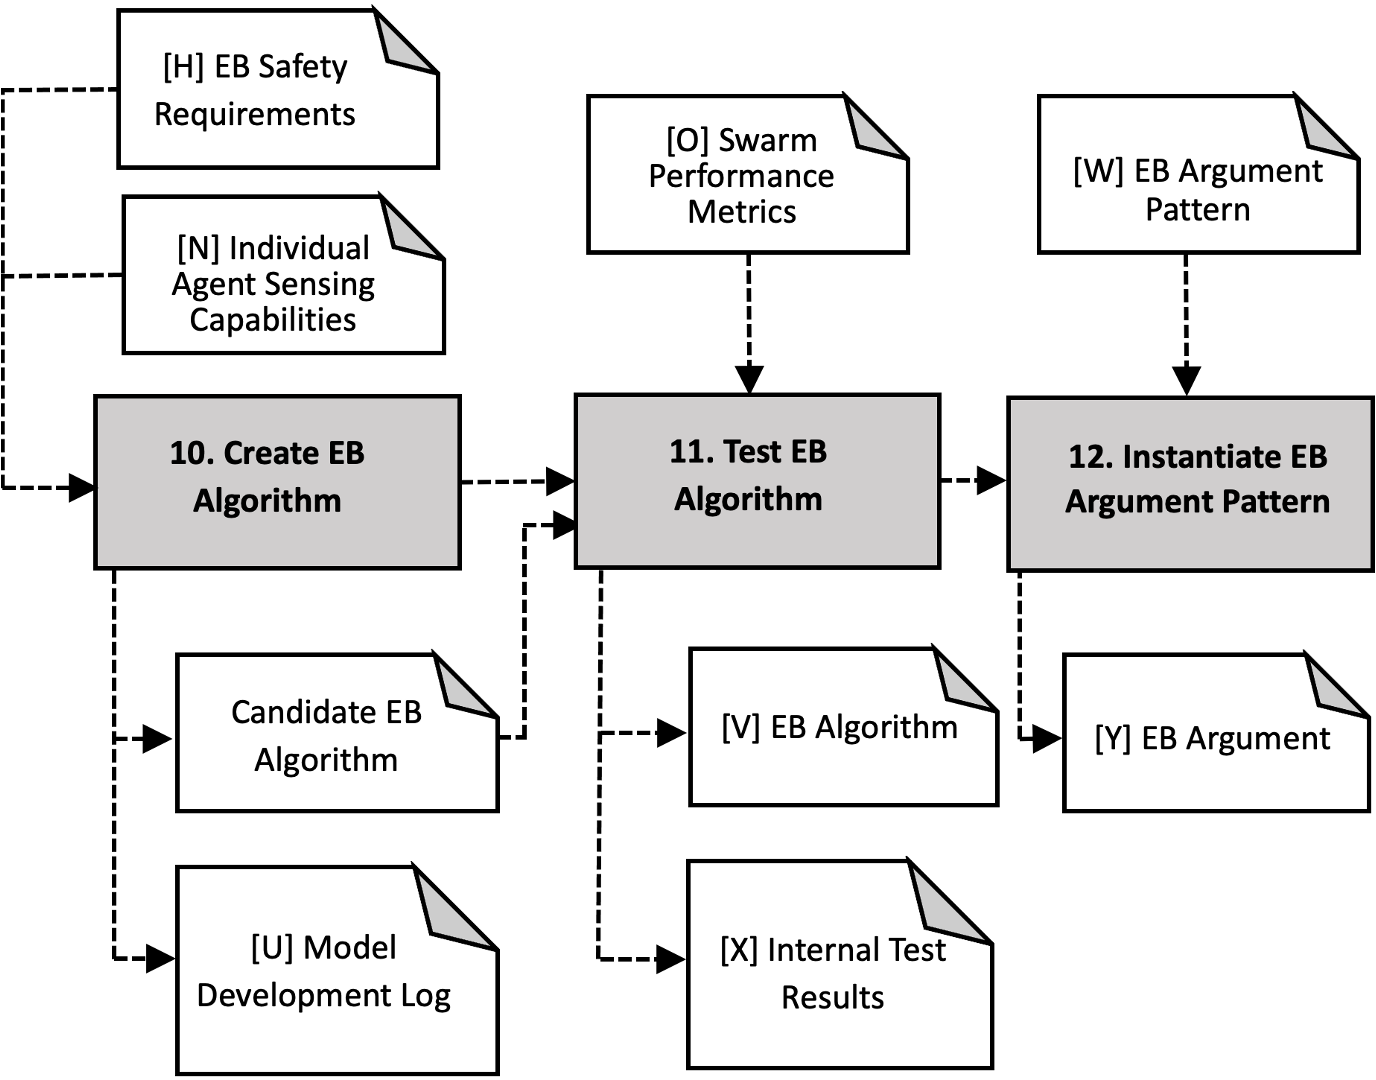
\includegraphics[width=0.5\textwidth]{figures/amlas-a-stage4-v2.png}%amlas-a-stage4.png
	\caption{Adapted AMLAS model learning process (right).}
	\label{amlas-a-stage4}
\end{figure}

In the design of an emergent behaviour algorithm, the challenge is in selecting behaviours at the individual level of the agent which give rise to the desired emergent behaviour at the swarm level. The original AMLAS application in Stage 4 focused on the creation, testing and instantiation of a machine learning model for a single system with no emergent behaviours to consider for a collective. In our adaptation of AMLAS for the robot swarm,  we step away from the machine learning paradigm to allow consideration for all possible optimization algorithms which may attain the target emergent behaviour.

\subsubsection*{Activity 10. Create EB Algorithm:}

Here we have two levels to consider: the individual level behaviour which is informed by individual agent sensing capabilities [N*] and the swarm level emergent behaviour which shall necessarily meet the safety requirements [H] defined in Stage 2. In the example of the cloakroom given in Section \ref{ex:cloakroom}, the target emergent behaviour for the swarm shall ensure that items are stored and retrieved by individuals. Performance requirements RQ1.1 and RQ1.2 specify an upper bound on the low/high impact collisions that a swarm shall experience in a given time frame. These requirements may be fulfilled by constraining the maximum velocity of individual robots, for example, or by ensuring that a robot has a camera or infra-red sensors which enable it to detect obstacles. The outputs from this activity follow the AMLAS framework, with a candidate emergent behaviour algorithm produced rather than a ML model. Output [U], the model development log, should log the rationale in the design process of the emergent behaviour algorithm.

\subsubsection*{Activity 11. Test EB Algorithm:}

In this activity, the candidate emergent behaviour will be tested against the swarm performance metrics [O] produced in Stage 3. Testing ensures that the emergent behaviour performs as desired with respect to the defined metrics and in the case where performance is above the accepted thresholds, the emergent behaviour algorithm will be produced as an output [V] of the activity. The internal test results [X] will also be an output from the testing process.

\subsection{Stage 5: Model Verification} \label{framework-stage5}
\noindent \textbf{\textit{[Lead:  WP4]}}\\ 
\noindent\textbf{\textit{Author Guidelines: 900–1800 words / 1–2 pages (maximum); \\Format/structure: Describe adapted AMLAS activities, inputs and outputs using cloakroom case study examples. Activities: 13; Inputs: H, P, V; Outputs: Z, AA}}\\
See Fig.~\ref{amlas-a-stage5} and Fig.~\ref{amlas-a-testbench}.	

% *****************
% GC Contribution, see table for qualities on `swarm' tab here:
% https://uob.sharepoint.com/:x:/r/teams/grp-TAS_Research2/Shared%20Documents/Verification/presentations/TrustQualities.xlsx?d=w4527b0bf0f4e49ab905d638dcb8c14ff&csf=1&web=1&e=8RW2vb

Inputs to the verification process are the [H] EB Safety Requirements, [P] Verification Scenarios (Test Generation) and [V] EB Algorithm. 
%
The verification method and assessment process within that method will be largely determined by the specifics of the safety requirements and examples from the cloakroom example will be used to illustrate the process. Some safety specifications lend themselves towards certain assessment methods due to the scenarios they prescribe.
%
For example, assessing the swarm system meets the requirements for performance given a motor fault injection [RQ1.6] may be easier to realise in physical or simulation based testing approaches, than constructing a reliable formal model of robot behaviour given the complex physical dynamics of a faulty wheel. 
%
However, when considering the adaptability requirements, a formal, probabilistic-based verification technique of the EB algorithm [V] is more suitable. For example, in [RQ2.1] analysis using a probabilistic finite state machine of the swarm behaviour tree, for example see \cite{Hoffmann2016,Calinescu2018}, could identify the dwell period within certain states. Monitors could be used to observe when agents enter a stationary state, e.g. \texttt{agent\_velocity=0 $\land $  t\_counter  $\ge$ 100}, and identify if time within that state exceeded some fixed value, and ascertain a probabilistic value to this metric.
%
These examples will now be expanded in more detail below.

\subsubsection{Verification Scenario (Test Generation) [P]}

In most cases there will be multiple, valid verification scenarios, also called test cases, applicable for each of the safety specifications. A `good test case' must be \emph{effective} at finding bugs or defects, \emph{efficient} in minimising the number of tests required, use resources \emph{economically} and be \emph{robust} to system changes~\cite{Fewster1999}. Using the EB Safety Requirements specification [H] and the principles of `good test cases', a few examples of potential scenarios and appropriate verification methods are explored in Table~\ref{tab:testgen}. 

\subsubsubsection{RQ1.1 Low Impact collisions}

For RQ1.1, relating to low impact collisions, suitable scenarios should consider a mix of both synthetic and physical testing to observe the safety compliance of the swarm controller. An important metric for assessing this safety requirement will be colllision detection which could be achieved either through on-board hardware sensors or indirectly through external monitoring, e.g. overhead camera and tracking system. Simulation is a valid verification method for RQ1.1 as testing time can be accelerated through parallelisation and test generation could be automated to include some randomisation and constrained randomisation whilst monitoring the collision detection metric. Physical testing, usually limited due to time and cost constraints, should be more prescriptive and should orchestrate scenarios that have a high probability of exercising the collision detection routine of the swarm agent controller ([V] EB Algorithm), for example forcing swarm agents to travel a narrow passage to elevate sarm density. 

Runtime verification can offer a solution to verifying systems that operate in large state-spaces, that may be intractable to verify at design time or through sampling the state space in testing. However, the choice or design of runtime oracle which provides the ground truth may require significant development, or innovative solutions~\cite{maple2020cyres}. However, for RQ1.1 of the swarm safety requirement this may be achieved with collision detection monitors, either implemented within the swarm robots or externally monitored through a tracking system, e.g. Vicon. Tracking with an external systems may be less reliable that physical sensing, e.g. accelerometer based collision detection, but being an independent system offers other assurances, being an independent evidence sosurce and protect against cascading failure that may occur due to collisions where the agents fail to report the collision event due to other failures, e.g. network connectivity.

\subsubsubsection{RQ2.2 Agent Movement}

For RQ2.2, which ensures agents move every 100 seconds outside the delivery area, a suitable verification metric could monitor the time agents are ouside a designated geospatial area (the delivery site) in addition to monitoring agent wheel speed. Scenarios should be biased towards these conditions by, for example, ensuring a sufficient number of agents outside the delivery area (by making the delivery area small or non-existent) and monitoring when wheel speed is zero for sufficiently long horizons to improve the likelihood of witnessing such an event by chance, e.g. see~\cite{chance2020agency}. Increasing the chance that such rare events occur can accelerate evidence gathering which could be done in this case, for example, by constraining the agents environment, increasing swarm density, or fault injecting to the collision sensors so valid movement actions are limited. 

Whereas RQ1.1 is only suitable for simulation and physical testing, RQ2.2 could use these techniques in addition to also using a formal verification anlaysis. A formal analysis could take the form of a probabilistic finite stste machine~\cite{Calinescu2018}, which would require a description of the agent states and the state transition proabilities. State transition probabilities can be derived from an action selection policy which, for this use case, can be derived from the swarm controller behaviour tree. Whereas testing based verification (physical, simulation, etc.) samples the input space, a formal analysis can prove a system property across the entire parameter range, which can be particularly beneficial in giving confidence in system compliance against the requirements. 


\subsubsection{Verification Testbench}

For simulation-based testing, a testbench can be used to orchestrate the `verify' task (stage 13 of AMLAS), see Figure~\ref{amlas-a-testbench}. The testbench operates by using a \emph{simulator} to test the \emph{Agent Controller} software ([V] EB Algorithm) against \emph{Static} and \emph{Dynamic} stimuli. These stimuli are formed from \emph{Scenery} and \emph{Actor Behaviour} components which could be, for example, a virtual warehouse with staff, other robots and controllable lighting presenting a typical scenario to the virtual swarm. The \emph{Swarm Requirements} are used to drive suitable experiment instantiation so that the stimuli provoke the intended behaviours in the swarm that will prove (or possibly disprove) the safety properties under observation. A coverage monitor will be used to check that all the requirements have sufficient evidence against each entry and, for dynamic testbench architectures, can even be used to drive additional test cases. 

In addition to requirements coverage, the there may also be coverage place on the Agent Controller code itself, ensuring that all code is executed as expected for each behaviour. Assertions Coverage is a third method by which safet assurance evidence can be gathered. Assertions are statements pertaining to system properties written in the form of a ruleset, for example "A swarm agent shall not collide with another swarm agent". Such an assertion can be monitored during verification activities, which is represented in the lower right section of the testbench. Through \emph{logging} the appropriate data channels, such as agent position and speed, and then analysing the data to perform \emph{Assertion Testing} either at runtime or offline, the swarm can be shown to comply with these assertions e.g. see~\cite{harper2021safety}. 

\begin{figure*}
	\centering
	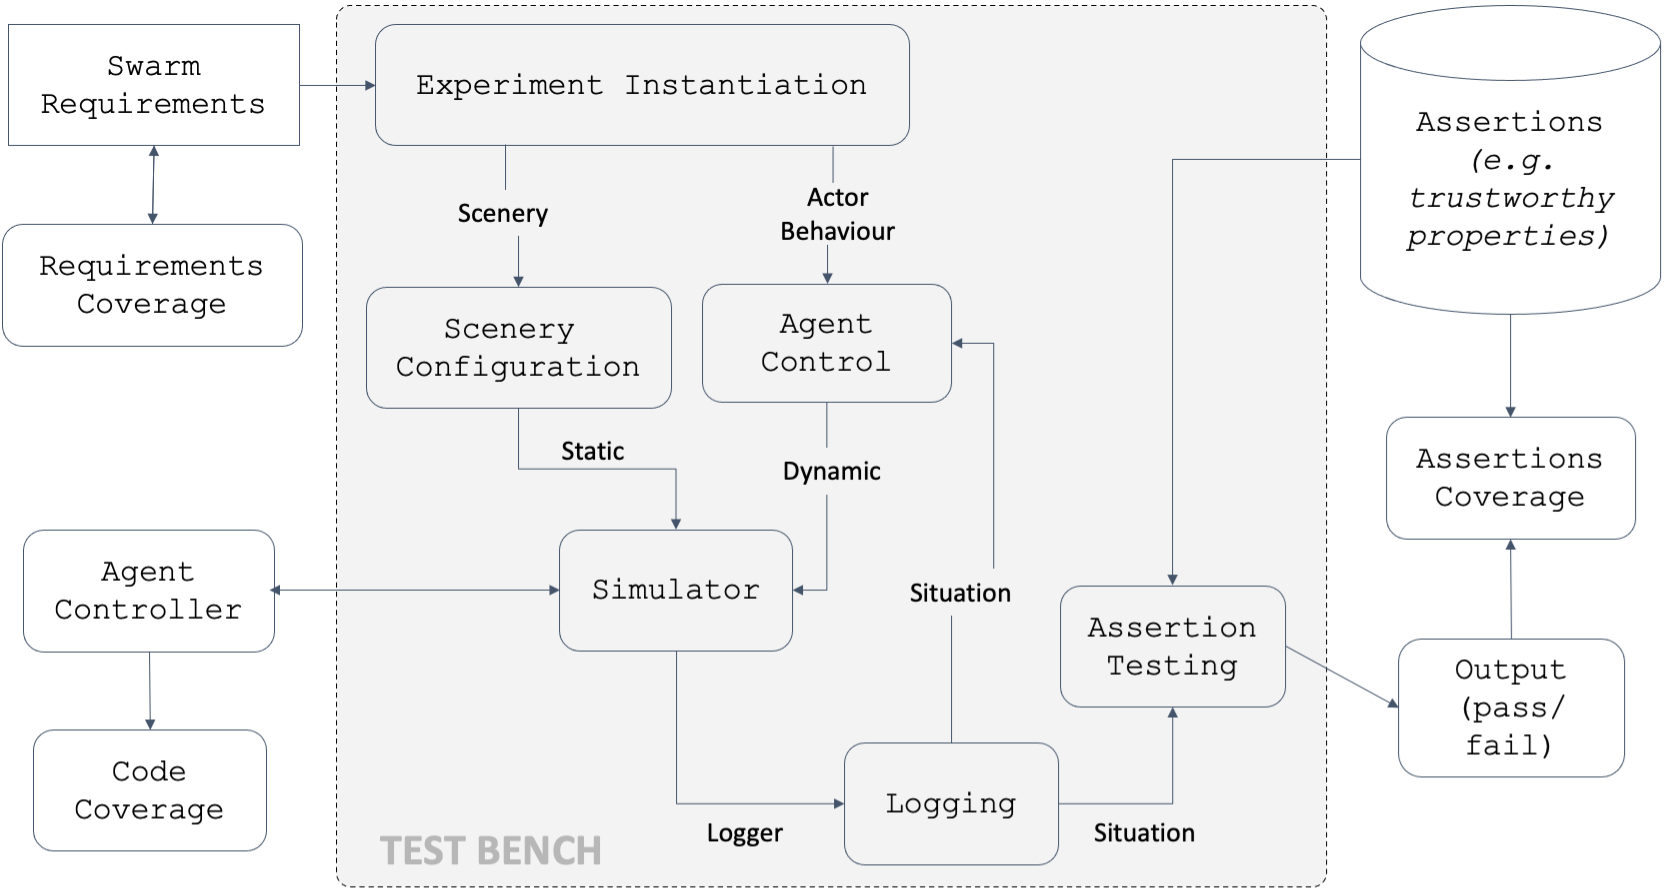
\includegraphics[width=1.0\textwidth]{figures/verification-testbench.png}
	\caption{Adapted AMLAS verification assurance process: test bench.}
	\label{amlas-a-testbench}
\end{figure*}


\begin{table*}[t]
\caption{Verification scenarios [P] and suitable methods.}\label{tab:testgen}
\centering
\begin{tabular}{llll}
\textbf{RQ}   & \textbf{Verification}  & \textbf{Verification} & \textbf{Scenario} \\ 
              & \textbf{Class}         & \textbf{Method}		  & 		          \\ 
\hline
1.1 	      & simulation 	   & constrained randomisation, directed tests & path intersection     \\
low impact    & physical testing   & prescriptive trial 				       & path intersection	 \\
collisions    & runtime		   & collision monitoring metric 		       & operational		 \\
\hline
2.2 	      & formal 	 	   & probabilistic finite state machine 	   & n/a      \\
movement      & simulation 	   & constrained randomisation, directed tests & task representative     \\
every 100s    & physical, runtime  & stationary monitoring metric 			   & operational		 \\
\hline
\end{tabular}
\end{table*}

\subsubsection{Verifiability & Visualisation}

Physical testing offers the opportunity to measure ground-truth..
Resolves the reality-gap to simulation...
Physical tends to take longer, cost more to acquire data...

Verifiability is the process by which the verification task can be achieved with less effort through implementation of useful metrics and processes prior to the  development stage, i.e. at design time. Much effort goes into verifying systems that have already been developed, but by thinking how system properties can be observed or measured during the design stage and implementing these, will allow for greater transparency and explainability of the system to verification engineers and regulators. This could be creating software inspection points~\cite{koopman2018toward} giving visibility of decisions or actions taken by the system in a human-readable format. 

Fig.~\ref{swarm_trust_spider} is an example of a safety visualisation spider graph for a swarm. By considering verifiability, monitors could be included into the system to monitor events such as \emph{Task Performance}, \emph{Agent Uptime} and \emph{Collision Avoidance} rate. If the average \emph{Idle Rate} of the swarm was monitored then operators could identify optimal operational agent numbers for the swarm, and either add or remove agents as a direct response to this metric, to give optimal task performance. By visualising \emph{Network Connectivity} operators can be reassured of this function to improve trust and adoption of the system and help debug system if error occur. 

\begin{figure*}
	\centering
	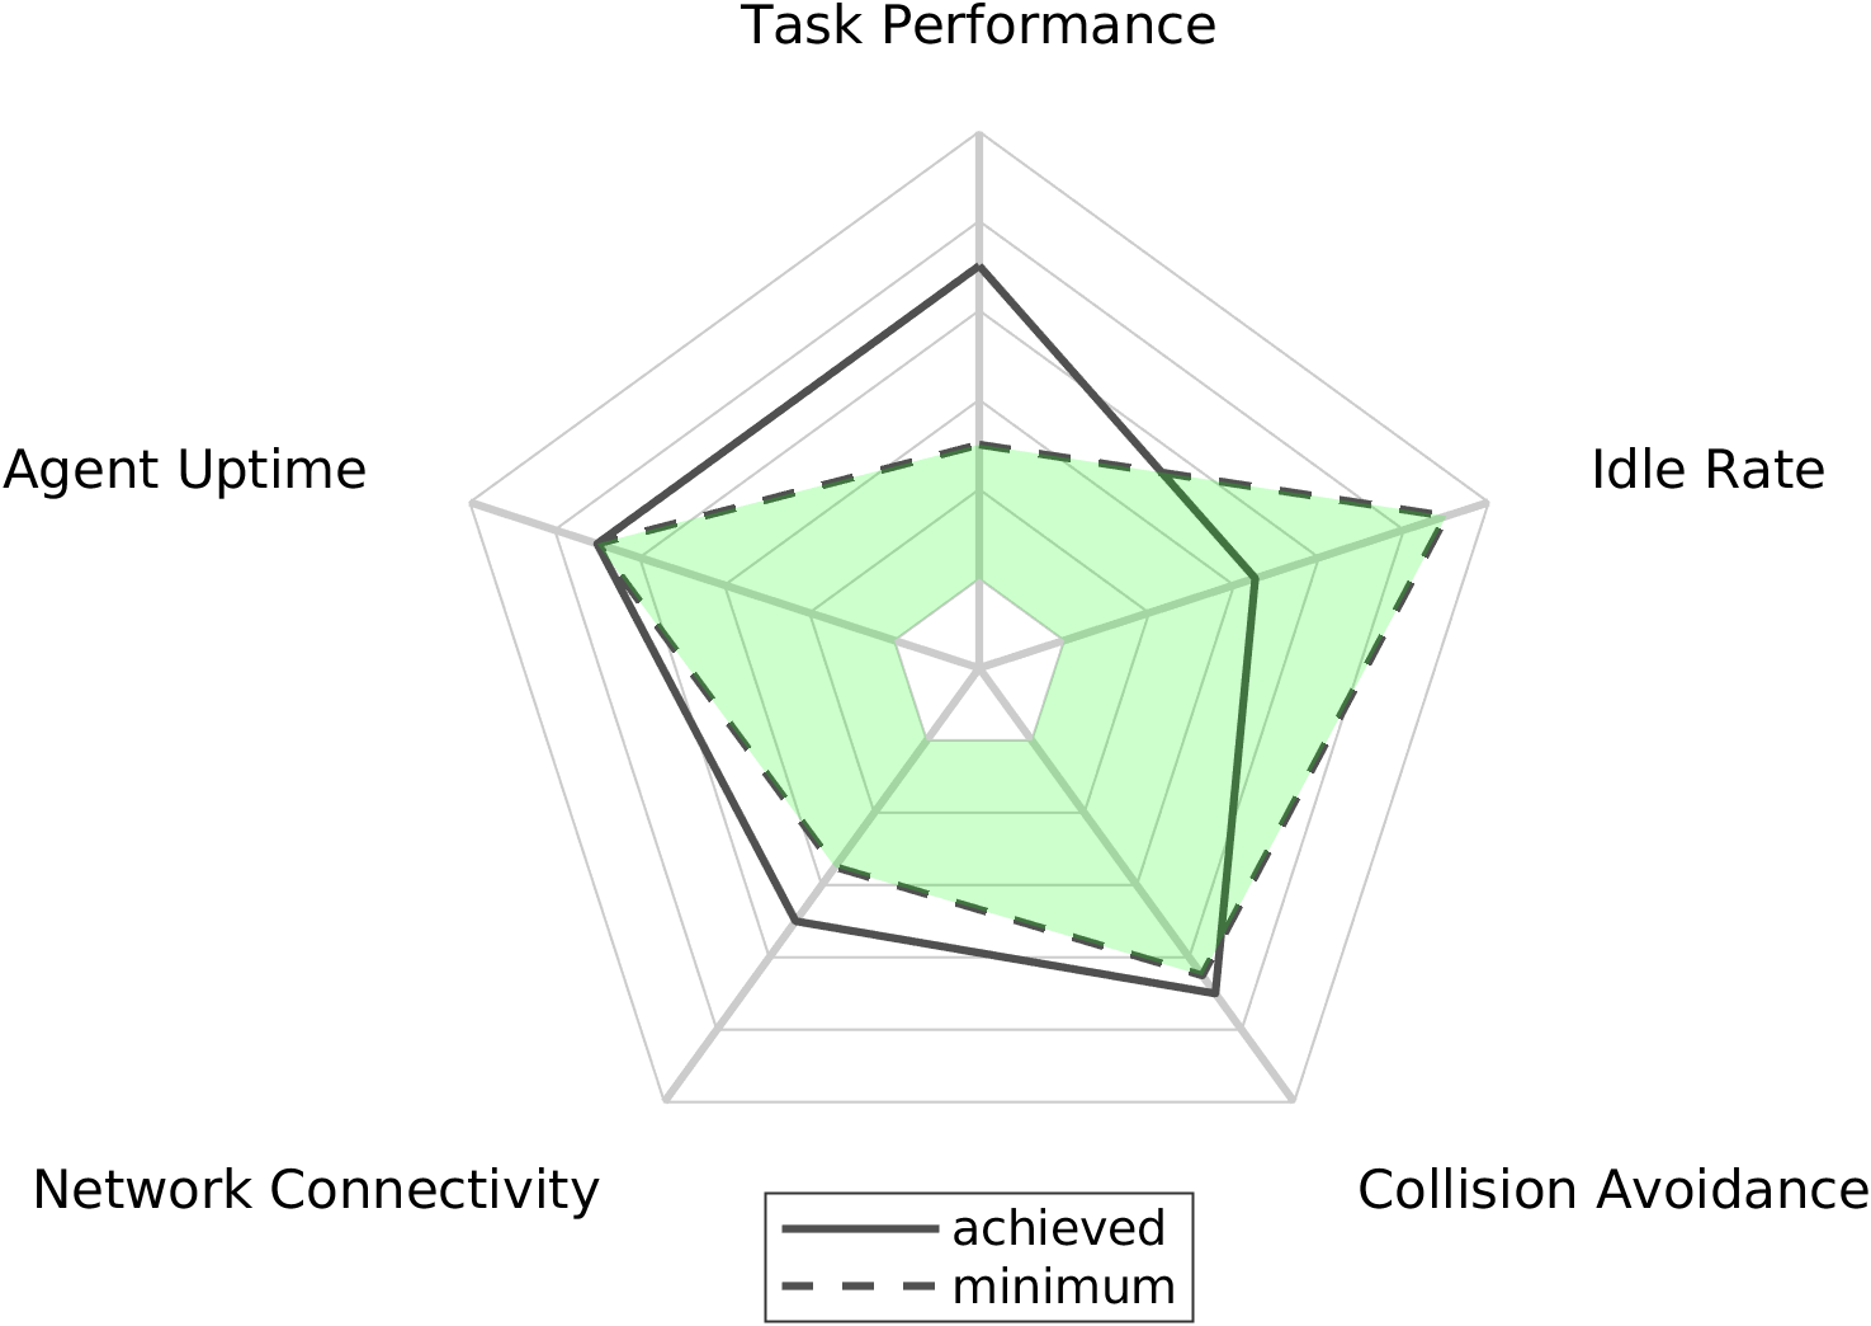
\includegraphics[width=1.0\textwidth]{figures/swarm_trust_spider.png}
	\caption{Visualising swarm safety properties.}
	\label{swarm_trust_spider}
\end{figure*}

%\begin{itemize}
%	\item Test bench for swarms
%	\item Probabilistic verification ideas
%	\item Simulation-based testing
%	\item Verifiability?
%\end{itemize}

\begin{figure*}
	\centering
	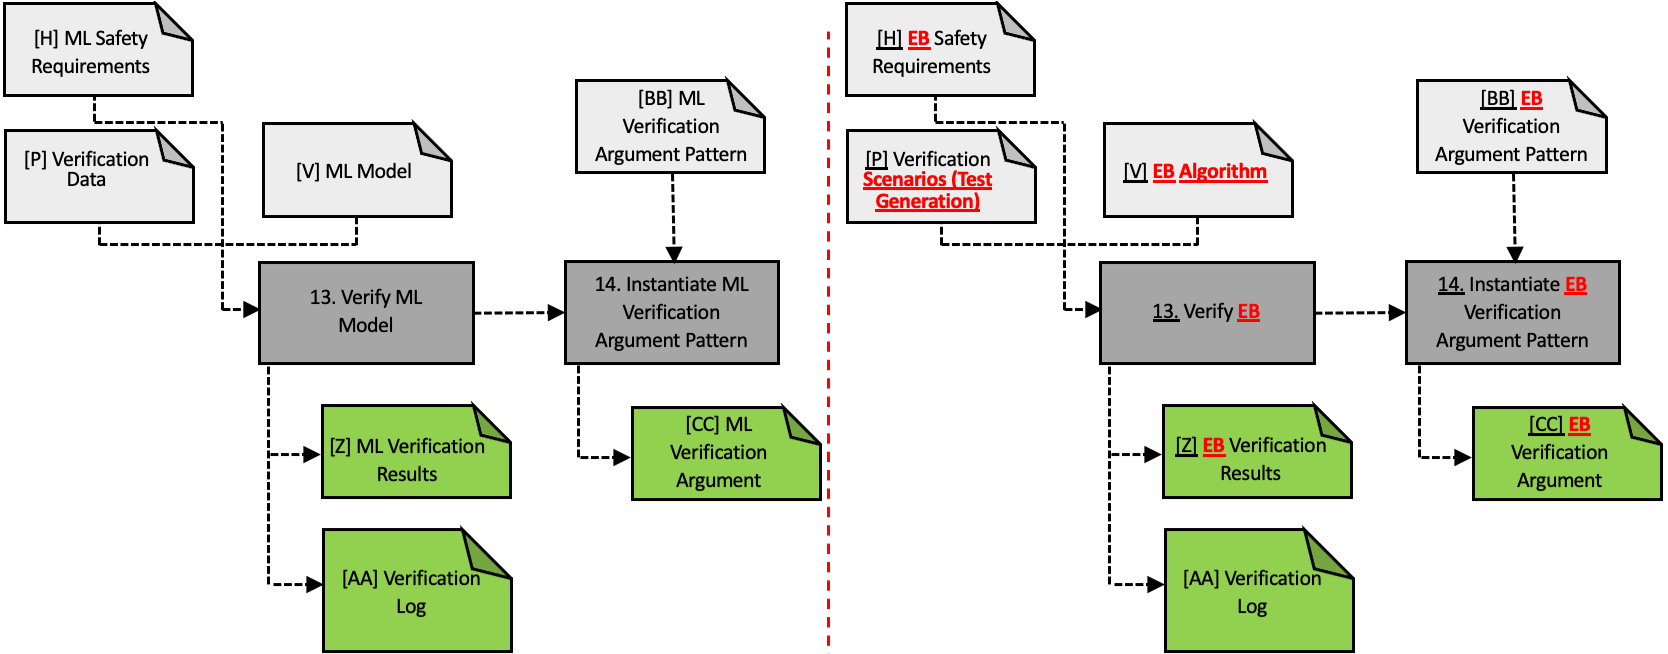
\includegraphics[width=1.0\textwidth]{figures/amlas-a-stage5.png}
	\caption{Adapted AMLAS verification assurance process (right).}
	\label{amlas-a-stage5}
\end{figure*}


\subsection{Stage 6: Model Deployment} \label{framework-stage6}
\noindent \textbf{\textit{[Leads:  WP4 \& WP5; Additional: WP3]}}\\ 
\noindent\textbf{\textit{Author Guidelines: 900–1800 words / 1–2 pages (maximum); \\Format/structure: Describe adapted AMLAS activities, inputs and outputs using cloakroom case study examples.\\ 
\noindent WP5 = (Activities: 15, Inputs: V, A, B, C, D, Outputs: DD), \\
\noindent WP4 = (Activities: 16, Inputs: EE, Outputs: FF), \\
\noindent WP3 = (Regulatory Considerations – 675 words / 0.75 page maximum)}}\\
See Fig.~\ref{amlas-a-stage6}
\begin{figure*}
	\centering
	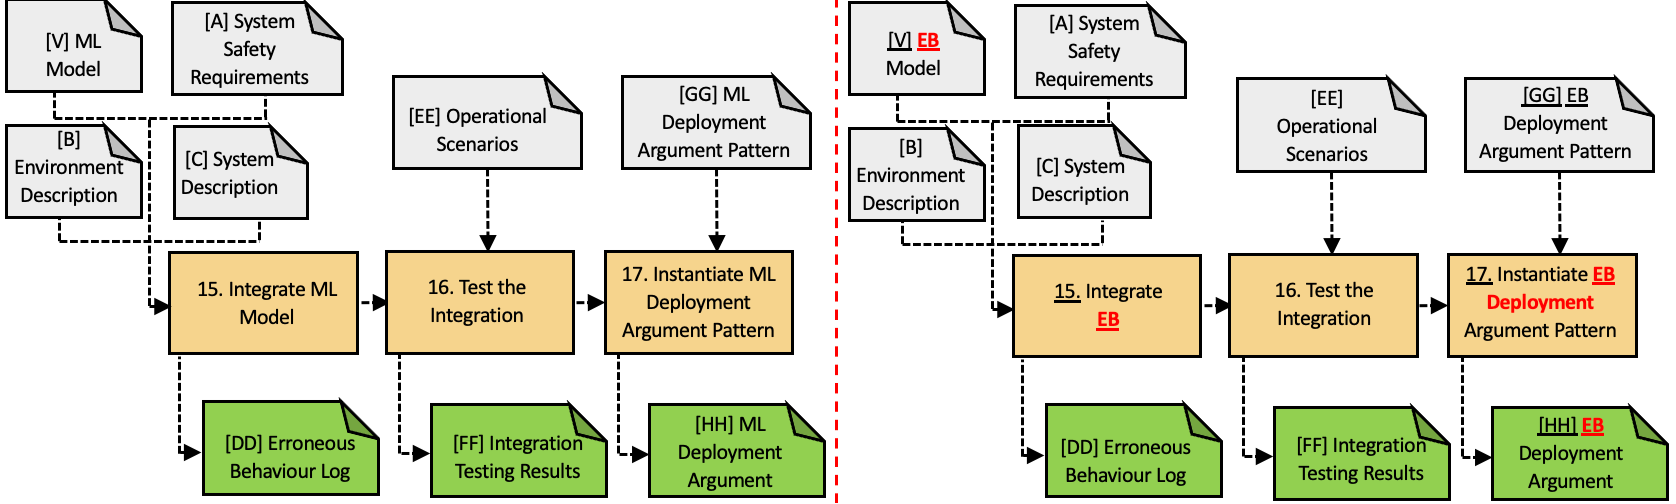
\includegraphics[width=1.0\textwidth]{figures/amlas-a-stage6.png}
	\caption{Adapted AMLAS model deployment assurance process (right).}
	\label{amlas-a-stage6}
\end{figure*}

\subsubsection*{Activity 15. Integrate EB}

With the emergent behaviour verified, the next step is to take the model [V] as well as the system safety requirements [V], environment description [B] and system description [C] and integrate the emergent behaviour with the system to be deployed. In this activity we use the inputs to this stage to educate the implementation of the emergent behaviour and anticipate errors we might expect in the interactions between agents and the overall emergent behaviour. Despite the rigorous validation and testing conducted in previous stages, there will still be a gap between the test environment and the intended, every day use, deployed scenario. The output, [DD] Model Development Log, captures these anticipated gaps between testing and reality and the differences in behaviour that might sprout from them.

For example, once physically deployed it may become apparent that large fluctuations in speed used to maintain performance while keeping the system safe for Humans, may in reality be too much of a draw on the agents batteries to get a reasonable lifetime out of each battery charge. To address this the behaviour may need to be tweaked to sacrifice some performance in the short term, reducing the rates of acceleration experienced by agents, in order to gain a longer battery life.

\subsubsection*{Activity 16. Test the Integration}

Once the initial integration is complete the physical implementation should undergo an additional round of testing in which the system will be observed in multiple operational scenarios, as specified in [EE].

\paragraph*{[EE] Operational Scenarios}

These operational scenarios should reflect the environment descriptions specified in [B], offering a real-world situations to examine the behaviour of the integrated system. The testing of the integrated system in these true-to-operation environments should be conducted in a safe manner. Ensuring that the entire multi-agent system can be shut down in an emergency, or providing shadow operators for groups of agents, taking over should the swarm behave erroneously.

In our cloakroom scenario, an example of [EE] may take the form of a small deployment of agents in a real but controlled coat storage area.

% Capture any integration issues

% provide a few environment examples

% Identify Erroneous behaviour expected and outlined in [DD], while simultaniously looking to catch/identify any issues of integration previously overlooked.

\paragraph*{[FF] Integration Testing Results}

Results from the integration testing will be reported here, detailing how the system performs against the safety requirements [H] specified in stage 2.

%\subsection{Stage 7: Assurance Case}
	
\section{Discussion and Conclusions} \label{discussion-conclusions}

\section*{Acknowledgments}
The work presented in this paper has been supported by the UK Engineering and Physical Sciences Research Council (EPSRC) under the grant [EP/V026518/1].

\appendices
\section*{Appendix A. Ethics matrices}
The content of the following tables has been developed through interdisciplinary discussions between the authors, and is informed by the authors’ preliminary interactions with members of the public and companies who may one day buy and deploy the system. The tables refer to the cloakroom use case unless otherwise specified. 

Please note that, at this early stage, these tables are only suggestive. More comprehensive discussions should be undertaken to ensure that they reflect the views of all stakeholders. Moreover, the tables will require continuous update after system deployment. 

\begin{landscape}

\begin{table}[]
\begin{tabular}{|p{0.15\textheight}|p{0.18\textheight}|p{0.18\textheight}|p{0.18\textheight}|p{0.18\textheight}|p{0.18\textheight}|}
\hline
Groups of beneficiaries & Physical benefits & Psychological benefits  & Financial/economic benefits   & Reputational benefits  & Legal benefits \\ \hline

Members of the public  &  & End users may enjoy a faster and more convenient service. 

End users may derive entertainment from interacting with robots. 

End users may become optimistic about or develop positive attitude towards technology. & Automation may allow end users to enjoy receiving the service at reduced cost. &  & End users may benefit from a reduced risk of property theft by human staff. \\ \hline

Trained humans  & The continual availability of agents in the swarm benefits human operators by reducing repetitive strain. & With the swarm system in place operators no longer need to remember where items were left, which in turn reduces the cognitive load of working within the cloakroom environment. & New jobs may become available to human workers as intermediaries between members of the public and robots (human-robot translators). & & 
 \\ \hline

Manufacturers &  &  & New jobs may become available for robot developers. Manufacturers may enjoy opportunities to develop patents for their technologies. & The quality of the system may be reflected in the manufacturers’ reputation. & Manufacturers may enjoy opportunities to develop patents for their technologies. \\ \hline

Company deploying the swarm &   &  & The company deploying the swarm may benefit financially from opportunities for better worker triage (e.g., investing more in workers for primary business function). The company may benefit from an automated solution without the need for expensive heavy infrastructures, made possible by the decentralized nature of swarms. The company may benefit from long-term financial savings from service automation. & The company deploying the swarm may be considered a technologically advanced company and develop a reputation as a trend setter.& Liability: Legal responsibility for errors in the system that cause harm to humans, property damage or loss may be moved to manufacturers.  \\ \hline
\end{tabular}
\caption{\label{tab:beneficence}Beneficence matrix}
\end{table}

\end{landscape}

\begin{landscape}
\begin{table}[]
\begin{tabular}{|p{0.10\textheight}|p{0.07\textheight}|p{0.20\textheight}|p{0.20\textheight}|p{0.20\textheight}|p{0.20\textheight}|p{0.20\textheight}|}
\hline
Groups of risk-exposed & Physical harms & Psychological harms & Data privacy harms  & Financial/economic harms   & Reputational harms  & Legal harms \\ \hline

Members of the public  & \textit{Addressed by technical requirements.} & Inexperienced users may experience psychological discomfort (stress) from interacting with a novel (not seen before) and complex (multi agent) system. 

The swarm unpredictable behaviour, due to the volume and decentralized nature of the system, could appear inefficient or untrustworthy to an inexperienced user. & Harms to end users may derive from personal data being collected, processed, and stored through the app. 

Harms may derive from personal data (users’ names, addresses, photos, videos) being stored on the agents and dispersed across agents in a decentralised manner. & Members of the public may experience financial/economic harms if their property is lost or damaged due to the non-explicitly guided (emergent) behaviour of agents. & Loss of property due to the non-explicitly guided (emergent) behaviour of agents may cause reputational harms on members of the public. & Liability (legal responsibility): Members of the public engaging in inappropriate interactions with the system may be considered legally responsible for injuries, accidents, damage or loss of property. \\ \hline

Trained humans  & \textit{Addressed by technical requirements.} & Managed behaviours of swarm agents that appear cohesive to inexperienced user may in fact be less efficient, and so frustrating to trained operators.

Increased cognitive overload from monitoring a multi-agent system, including in scenarios that involve ethically-relevant decisions. & Harms to operators may derive from personal data being collected, processed, and stored through the app.

Harms may derive from personal data (operators’ names, addresses, photos, videos) being stored on the agents and dispersed across agents in a decentralised manner. & Current workers within the use case space may be replaced by robots. & Moral responsibility: Operators may be morally blamed for errors in the system that cause harm to humans, property damage or loss. & Liability (legal responsibility): Errors in the system that cause harm to humans, property damage or loss may be attributed to human operators. \\ \hline

Manufacturers & \textit{Addressed by technical requirements.} &  Manufacturers may experience moral distress, which is defined as “the combination of (1) the experience of a moral event, (2) the experience of `psychological distress’ and (3) a direct causal relation between (1) and (2)” \cite{morley2019moral}. Moral distress may derive from  making design decisions to automate functions that would normally require human interpretation and ethical judgment, or from reflecting on the ethical and societal implications of system deployment (e.g., machines replacing humans in the workplace; systems being repurposed to kill targets in military applications). & & Manufacturers may incur in additional costs due to system malfunctioning. & Moral responsibility: Manufacturers may be morally blamed for errors in the system that cause harm to humans, property damage or loss. & Liability (legal responsibility): Errors in the system that cause harm to humans, property damage or loss may be attributed to manufacturers. \\ \hline

Company deploying the swarm & \textit{Addressed by technical requirements.}  &  & & Managed behaviours of swarm agents that appear cohesive to inexperienced users may in fact be less efficient, and so may increase costs for the company deploying the system.

The company deploying the system may experience financial/economic harms if accidents or injury happen or if property is lost or damaged due to the non-explicitly guided (emergent) behaviour of agents. & Moral responsibility: The company deploying the system may be morally blamed for errors in the system that cause harm to humans, property damage or loss. & Liability (legal responsibility): Errors in the system that cause harm to humans, property damage or loss may be attributed to the company deploying the system. \\ \hline 
\end{tabular}
\caption{\label{tab:maleficence}Non-maleficence matrix}
\end{table}


\end{landscape}


\begin{landscape}
\begin{table}[]
\begin{tabular}{|p{0.10\textheight}|p{0.35\textheight}|p{0.35\textheight}|p{0.35\textheight}|}
\hline
Groups of autonomy risk-exposed  & Personal choice & Informed consent & Meaningful control \\ \hline

Members of the public  & Constraints on the personal choice of members of the public occur if there is not a human (non-automated) alternative to use the service (ability to opt out).

The emerging behaviour of the swarm could constrain end users’ options to access critical paths (e.g., to travel to urgent location safely). & Members of the public cannot provide valid consent if they are not given information about the system functioning and capabilities, tailored to their level of understanding, including information about the swarm’s emerging behaviour, and about how their personal data will be collected, processed, stored, and shared within the swarm. 

Members of the public cannot give valid consent if the system has properties (e.g., biomimetic features) that deceive them and exploit their trust heuristics. &   Members of the public cannot have meaningful control over the system if they are not adequately trained.

Members of the public cannot have meaningful control over the system if they do not have access to human readable information about the system and scenario at any given time.

Members of the public cannot have meaningful control over the system if they do not have the ability to physically interact with or intervene on the system and scenario at any given time.

Members of the public cannot have meaningful control if they cannot provide contextual awareness to the system when the system lacks/requires it.

In large swarms, due to the volume of the system, members of the public cannot have meaningful universal control beyond having an emergency stop that turns the whole system on/off. \\ \hline

Trained humans  & Constraints on the personal choice of operators occur if they are not free to decide whether to interact with the system to provide the service (particularly relevant at time of transitions from a non-automated to an automated service). 

The emerging behaviour of the system could constrain operators’ options to access critical paths (e.g., to travel to urgent location safely).

The emerging behaviour of the system could interfere with business policies in a way that constrains operators’ options (e.g., if a business policy prohibits trained humans to step over a robot or walk in an area where the density of agents is high, but because of its emergent behaviour the swarm behaves unexpectedly, hence leading the operator to violate that policy). & Operators cannot provide valid consent if they are not given information about the system functioning and capabilities, tailored to their level of understanding and monitoring needs, including information about where responsibility lies in case of system malfunctions. & Operators cannot have meaningful control over the system if they are not adequately trained.

Operators cannot have meaningful control over the system if they do not have access to human readable information about the system and scenario at any given time.

Operators cannot have meaningful control over the system if they do not have the ability to physically interact with or intervene on the system and scenario at any given time.

Operators cannot have meaningful control if they cannot provide contextual awareness to the system when the system lacks/requires it.

In large swarms, due to the volume of the system, operators cannot have meaningful universal control beyond having an emergency stop that turns the whole system on/off. 

\\ \hline

Manufacturers & Constraints on the personal choice of manufacturers occur when they are not free to decide how to design and develop the system due to resource limitations, institutional constraints, commercial interests or market imperatives. & Manufactures cannot give valid consent to system deployment if they do not have access to or do not understand the inner decision making of the system. & Manufacturers cannot have meaningful control over the system if the behaviour resulting from the system’s specifications does not reflect the manufacturers’ intentions. \\ \hline

Company deploying the swarm & Constraints on the personal choice of the company deploying the system may occur if the company is not free to decide whether to adopt the system to provide the service (e.g., because of automating the service is the only economically viable option or due to new government regulations). & The company deploying the system cannot provide valid consent if they are not given information about the system functioning and capabilities, tailored to their level of understanding, including information about the swarm’s emergent behaviour, and where responsibility lies in case of system malfunctions. 

The company deploying the system cannot give valid consent if the system has properties (e.g., biomimetic features) that deceive them and exploit their trust heuristics. &  The company deploying the system cannot have meaningful control if it does not have trained humans, and if the conditions for trained humans’ meaningful control are not met.

The company deploying the system cannot have meaningful control if it does not have a detailed documentation of how the system works, failures to expect, typical and atypical system behaviour etc.\\ \hline 
\end{tabular}
\caption{\label{tab:autonomy}Respect for autonomy matrix}
\end{table}

\end{landscape}


\begin{landscape}
\begin{table}[]
\begin{tabular}{|p{0.15\textheight}|p{0.18\textheight}|p{0.18\textheight}|p{0.18\textheight}|p{0.18\textheight}|p{0.18\textheight}|}
\hline
Groups of justice risk-exposed & Access to the system & Use of the system & Distribution of benefits and burdens & Redress & Punishment \\ \hline

Members of the public  & Unfair treatment of members of the public may occur if there is not a human (non-automated) alternative to access the service (ability to opt out). & Unfair treatment may occur if there are barriers that prevent some members of the public to use the system (e.g., boxes are too low, hence preventing people with mobility impairment from depositing/retrieving their coat).

Unfair treatment may occur if the system does not recognize some authorized* members of the public due to their characteristics (wheelchair users, different ethnicities etc.) *authorized = with Bluetooth turned on.

Unfair treatment may occur due to the lack of a priority order for coat depositing and retrieval (procedural justice). & Members of the public may be unfairly treated if distribution of benefits and burdens is inequitable (e.g., if they are among the risk-bearers but not among the beneficiaries of the development and deployment of the system). & Unfair treatment of members of the public may occur if there is no mechanism for redress in case of system malfunction that leads to injuries, accidents, property damage or loss, or violation of any ethics requirement affecting them. & Members of the public may be treated unfairly if there is no appropriate punishment for certain kinds of trained humans’, manufactures’ or companies’ wrongful acts (e.g., negligence) that harm them. \\ \hline

Trained humans  & Unfair treatment may occur if there are barriers that prevent some trained humans to perform the job/deliver the service (requirement of reasonable adjustments, especially in transition period). &  Unfair treatment may occur if the system does not recognize some authorized* trained humans due to their characteristics (wheelchair users, different ethnicities etc.) *authorized = with Bluetooth turned on. & Trained humans may be unfairly treated if distribution of benefits and burdens is inequitable (e.g., if they are among the risk-bearers but not among the beneficiaries of the development and deployment of the system). & Unfair treatment of trained humans may occur if there is no mechanism for redress in case of system malfunction that leads to injuries, accidents, damage or loss, or violation of any ethics requirement affecting them. & Trained humans may be treated unfairly if there is no appropriate punishment for certain kinds of end users’, manufactures’ or companies’ wrongful acts (e.g., negligence) that harm them. \\ \hline

Manufacturers & & & Manufacturers may be unfairly treated if distribution of benefits and burdens is inequitable (e.g., if they are overburdened by inequitable risk bearing). & Mechanisms for redress should be in place to rectify any injustice/damage (e.g., reputational harm) experienced by manufacturers due to malicious use. & Manufactures may be treated unfairly if there is no appropriate punishment for certain kinds of end users’, trained humans’, or companies’ wrongful acts (e.g., negligence) that harm them. \\ \hline

Company deploying the swarm & Unfair competition may occur if the costs of automating the service or replacing faulty agents make the swarm only affordable to large and established businesses. & & The company deploying the system may be unfairly treated if distribution of benefits and burdens is inequitable (e.g., if they are among the risk-bearers but not among the beneficiaries of the development and deployment of the system) \textit{[this is if we think of the company as the end user with respect to the developers]}. & Unfair treatment of the company deploying the system may occur if there is no mechanism for redress in case of system malfunction that leads to injuries, accidents, damage or loss, or violation of any ethics requirement affecting them \textit{[this is if we think of the company as the end user with respect to the developers]}. & The company deploying the system may be treated unfairly if there is no appropriate punishment for certain kinds of end users’, trained humans’, or manufactures’ wrongful acts (e.g., negligence) that harm them. \\ \hline 
\end{tabular}
\caption{\label{tab:justice}Justice matrix}
\end{table}

\end{landscape}


\section*{Appendix B. Regulation tables}

\begin{landscape}
\begin{table}[]
    \centering
    \begin{tabular}{|p{0.3\textheight}|p{0.35\textheight}|p{0.35\textheight}|}
\hline
\textbf{Structural Sources of Sociotechnical Risk:} Risks arising from interdependencies and interactions between different technical and social structures & \textbf{Risk scenario example} & \textbf{Regulatory Requirements} \\
\hline
\textbf{Disruption amplifiers} “System features which cause disruptions or failures to enlarge, expand or develop into more critical situations which are harder to deal with or recover from”. \cite{macrae2021learning}. Disruption amplifiers may also be thought of as a type of “interactive complexity”, where components may interact in unanticipated ways, perhaps because of failures or just because no designer anticipated the interactions that could occur \cite{perrow1999normal}. & A disruption or failure in one part of the swarm system (such as a fault in the upward facing camera) prevents one individual swarm agent responding to a perceived hazard, which can dramatically enlarge by impacting the performance of other swarm agents in ways that are hard to predict. For instance, the agent with the camera failure (which still think it has a box) might be trying to take preference over other robots, and might clutter up environment its working in, taking up the space of others. & \textbf{Identification and prevention of disruption amplifiers.} The system shall/should be able to identify features which cause disruptions or failures and prevent these from enlarging, expanding, or developing into more critical situations which are harder to deal with or recover from. For instance, an agent with a functioning radial camera can instruct the agent with the faulty camera that there is no box on its head.\\
\hline
\textbf{Failure cascades} “Structural characteristics that allow interlinked failures to cascade rapidly through interdependent functions of a system with few opportunities for identification or intervention”. \cite{macrae2021learning}. Failure cascades may also be thought of as a type of “tight coupling”, wherein a failure cannot be isolated but brings about other failures that cascade through the system \cite{perrow1999normal}. & A fault in one agent can cause other agents to fail in some way. For instance, one agent detects its position in the deposit site, and the second agent communicates this information to a third agent (with a message) that it detects another agent in the deposit space. However, this communication message fails and fails to distribute to the rest of the swarm. As a result, the agents who have not received the message start taking preference over others in that space, resulting in a clump of agents in that space and stopping those with garments travelling to the box drop off zone. & \textbf{Identification and prevention of failure cascades.} The system shall/should be able to identify structural characteristics that cause interlinked failures to cascade. This might come in the form of using the verification process to find issues in the system’s behaviour tree and issues in the system’s emergent behaviour. It might also come in the form of having an adequate density of robots in your environment is going to give you multiple paths and pieces of information or actionable intelligence for the agents to use (see the ‘environmental density of objects’ requirement above in the section titled: Human Safety requirements for the cloakroom).\\
\hline
\textbf{Vigilance dependencies}
“System functions that rely on active, real-time, moment-by-moment human vigilance to monitor automated behaviour and detect and address failures”. \cite{macrae2021learning} & If an individual swarm operator does not remain attentive to the monitoring of faulty swarm behaviour, they may not be able to intervene in time if the system fails. & \textbf{State of vigilance}
The system shall/should not be predicated on moment-by-moment and real-time monitoring of individual human operators. Instead, a assessment should be designed to nurture awareness activities and identify a vigilance state of the operators that is reasonable, rather than driving real-time vigilance, and to deliberate as to whether two or more people are needed to monitor the system. For instance, two or more people may be required to monitor the swarm during busy parts of the day/time of the event.\\
\hline
\textbf{Test permeabilities}
“New iterations of developmental or operational autonomous systems are released for testing into the public domain with few safety controls, criteria, or assurance processes”. \cite{macrae2021learning} & If there are no processes in place for human operators to request or conduct tests that meet a set of performance standards, then weaknesses in real-world behaviour will go unnoticed. & \textbf{Creation of test permeabilities} The system shall/should create test permeabilities (e.g., safety assessments or safety requirements) that allows new or updated systems to be rapidly and regularly released into the public cloakroom. \\
\hline
    \end{tabular}
    \caption{Regulation Table 1}
    \label{tab:reg_1}
\end{table}
\end{landscape}

\begin{landscape}
\begin{table}[]
    \centering
    \begin{tabular}{|p{0.3\textheight}|p{0.35\textheight}|p{0.35\textheight}|}
    \hline
   \textbf{Organisational Sources of Sociotechnical Risk:} Risks arising from social processes, organising activities and human and contextual factors & \textbf{Risk scenario example} & \textbf{Regulatory requirements}\\
   \hline
   \textbf{Invisible Automation.} “Weaknesses or gaps in processes that maintain awareness, provide insight and issue alerts regarding the status, activities, and decisions of automated systems”. \cite{macrae2021learning} & A swarm agent has gone ‘rogue’ and is away from the rest of the swarm AND has a significant error. However, there is no alerting process in place to inform human operators that the agent has the error. Because of this, it is unlikely that the operators will see the error message. Although the rest of the swarm may be able to continue to perform efficiently without the rogue agent, serious safety incidents could take place which may be going unnoticed (for instance, if a fault with the agent’s obstacle avoidance system is not detected the agent has the potential to bump into people’s shins).	& \textbf{Translucency around error reporting.} The system shall/should not create and hide errors (errors which can be nearly invisible or silent). Further to this, swarm operators could be provided with a mobile phone application that allows them to push a button and report the error.\\
   \hline
   \textbf{Governance gaps} “Gaps in organizational processes and systems that set standards for safety, monitor safety performance, and initiate action to address safety deficiencies”. \cite{macrae2021learning} & A swarm operator may have no safety management system in place to govern and assure the operational safety of the swarm system. &\textbf{Access to governance and standards.} The system shall/should have adequate resources for swarm operators to draw upon in governing and assuring the operational safety of the swarm. For example, having a safety plan or a standard for operating procedures that set out roles, responsibilities, and processes for the analysis and management of risk in its operations.
   \\
   \hline
   \textbf{Regulatory voids} “Absence of regulatory requirements, performance standards and associated oversight activities to assure the safe development, testing, deployment, and operation of automated systems”. \cite{macrae2021learning} & A swarm system may be subject to little regulatory oversight with no regulatory system in place by the company/local councils for monitoring safety performance.&
   \textbf{Regulative mechanisms.} The system shall/should help to identify relevant regulative mechanisms that regulate probabilistic risks and unpredictable phenomena on a local scale. \\
   \hline
   \textbf{Supervisory degradation} “Reduced or inadequate organizational arrangements to support, monitor, and assure the activities of supervising automated systems”. \cite{macrae2021learning} & The organisation has instituted no routine process or automated system to monitor swarm operator vigilance and reduced the number of operators per cloakroom environment from two to one, reducing the cognitive capacity available to monitor both the swarm graphical user interface and the environment. &	\textbf{Supervision.} The system shall/should develop a formalized or automated system to monitor the vigilance of swarm operators. Also, swarm operator shifts should be around 8 hours with a requirement to take a 20 - 40minute break after 4 hours of continuous monitoring. \\
   \hline
   \textbf{Competency limits} “Limitations or gaps in the roles, expertise, and experience available for analyzing and managing all aspects of safety across the development and deployment of an automated system”. \cite{macrae2021learning} & The cloakroom does not have a dedicated safety team or personnel with responsibility for managing the operational safety of its swarm. & \textbf{Safety expertise and Leadership} The system shall/should request that the organisation have a safety team in place, who have safety responsibilities combined with operational leadership responsibilities and relevant competencies made explicit through their roles.\\
   \hline
    \end{tabular}
    \caption{Regulation Table 2}
    \label{tab:reg_2}
\end{table}
\end{landscape}

\begin{landscape}
\begin{table}[]
    \centering
    \begin{tabular}{|p{0.3\textheight}|p{0.35\textheight}|p{0.35\textheight}|}
        \hline
        \textbf{Technological Sources of Sociotechnical Risk:} Risks arising from the capabilities, affordances and constraints produced in and by material technologies & \textbf{Risk scenario example} &	\textbf{Regulatory requirements} \\
        \hline
        \textbf{Automation immaturity} “Automated systems regularly encounter situations, objects or hazards that are not recognized or are beyond the system’s capabilities, leading to frequent failures”. \cite{macrae2021learning} & Camera systems may not have been designed to reliably recognise humans and because a hybrid system is being implemented (i.e., one that also uses Bluetooth to provide an approximate position of the human alongside the cameras) there is a difficulty that the hybrid system will only work if people have the smart phone application and the app is active. & \textbf{Automation maturity.} The system shall/should place restrictions on environments and place rules and regulations on people without a smart phone from entering that environment which has autonomous agents inside. Overall, the system shall/should produce guidelines that helps developers and operators to effectively test automation maturity in their swarm.\\
        \hline
        \textbf{Safety capability constraints} “Technical features that reduce or constrain the safety capabilities of a system in order to optimize other aspects of system performance, efficiency, or experience”. \cite{macrae2021learning} & The swarm system is unable to activate an emergency stop in circumstances where a collision was determined to be imminent in order to reduce the frequency of sudden stopping. For instance, the swarm has been designed to temporarily ignore perceived hazards so as to smooth the swarm’s motion, delaying avoidance action (e.g., for 1 second) in an attempt to reduce excessive stopping. & \textbf{Open capability.} The system shall/should add flexibility to the safety capabilities of its system in operating situations, also enabling operators to access, hear and read the exact type of information which is desirable to the operator and ensure that nothing is encrypted.\\
        \hline
        \textbf{Hazard masking} “Technical processes or features that result in hazards being inadvertently hidden, disguised, or rendered ambiguous”. \cite{macrae2021learning} & The design of the perception and prediction systems may be designed to inadvertently delete or overwrite the presence of potential hazards. For instance, the system was designed with a limited memory: if one agent has important information about a hazard but that information is deleted every ten seconds then critical information gets lost (not propagated properly to operators) & \textbf{Non-masking of hazards} The system shall/should not allow the company or operator to consider masking technical processes, components or features. Further to the solution of the swarm having a “collective memory” \cite{wilson2022information} as discussed above, a further solution for this risk could be the recording and storing of all information on a large database covering the performance of the swarm during its period(s) of operation.\\
        \hline
        \textbf{Autonomy reliance } “Dependence on autonomous functionality for technical safety protections and controls, to the exclusion of other lower-technology components that could provide safety redundancy”. \cite{macrae2021learning} & The swarm system relies solely on its own crash avoidance software to provide all hazard detection and avoidance functions, but the independent agent emergency obstacle avoidance function was disabled. &	\textbf{No self-reliance on internal infrastructure.} The system shall/should not only alert human operators that the emergency obstacle avoidance system is disabled/enabled, but that there may also be a “low tech” solution to the problem, such as putting bumpers on individual agents or putting them in ‘”zones”.\\
        \hline
    \end{tabular}
    \caption{Regulation Table 3}
    \label{tab:reg_3}
\end{table}
\end{landscape}

\begin{landscape}
\begin{table}[]
    \centering
    \begin{tabular}{|p{0.3\textheight}|p{0.35\textheight}|p{0.35\textheight}|}
         &  \\
         & 
    \end{tabular}
    \caption{Caption}
    \label{tab:my_label}
\end{table}
\end{landscape}

\begin{landscape}
\begin{table}[]
    \centering
    \begin{tabular}{|p{0.3\textheight}|p{0.35\textheight}|p{0.35\textheight}|}
         &  \\
         & 
    \end{tabular}
    \caption{Caption}
    \label{tab:my_label}
\end{table}
\end{landscape}

\bibliographystyle{IEEEtran}
\bibliography{AssuranceFWK-Swarms-Bibliography}

\newpage

\vfill

\end{document}


